\documentclass[a4paper,11pt]{report}
\usepackage[utf8]{inputenc}
\usepackage[T1]{fontenc}
\usepackage{todonotes}
\usepackage{appendix}
\usepackage{longtable}
\usepackage{amsmath}
\usepackage{amssymb}
\usepackage{tikz}
\usepackage{pgf}
\usepackage{geometry}
\usepackage{paralist}
\usepackage{hyperref}
\usepackage[format=hang]{subfig}
\usepackage{graphicx}
\usepackage{caption}
\usepackage{color}
\usepackage{float}
\usepackage{natbib}
\usepackage{apalike}
\usepackage[svgnames]{color}
\usepackage{commath}
\usepackage{listings}
\usepackage[boxed,ruled,lined,algochapter]{algorithm2e}
\usepackage[boxed,ruled,lined,algochapter]{algorithmic}



\newcommand{\Colin}[0]{\textsc{Colin }}

\pagenumbering{roman}
\geometry{a4paper,left=25mm,right=25mm, top=20mm, bottom=20mm} 

\linespread {1.5}

\let\oldsqrt\sqrt
\def\sqrt{\mathpalette\DHLhksqrt}
\def\DHLhksqrt#1#2{%
\setbox0=\hbox{$#1\oldsqrt{#2\,}$}\dimen0=\ht0
\advance\dimen0-0.2\ht0
\setbox2=\hbox{\vrule height\ht0 depth -\dimen0}%
{\box0\lower0.4pt\box2}}

\usetikzlibrary{calc}
\usepgfmodule{plot}
\usepgflibrary{plothandlers}
\usetikzlibrary{mindmap}
\usetikzlibrary{trees}
\usetikzlibrary{arrows}
\usetikzlibrary{automata}
\usetikzlibrary{positioning}
\usetikzlibrary{decorations}
\usetikzlibrary{backgrounds}
\usetikzlibrary{decorations.pathreplacing}



\bibliographystyle{apalike}


\makeatletter
\@addtoreset{lstlisting}{chapter}
\@addtoreset{table}{chapter}
\@addtoreset{figure}{chapter}
\makeatother

\begin{document}


\begin{titlepage}

\begin{center}
\ \\
\vspace{100pt}
\Huge{\textbf{Colin}}

\Large{User Manual for version 0.2.0-0
}

\vspace{100pt}
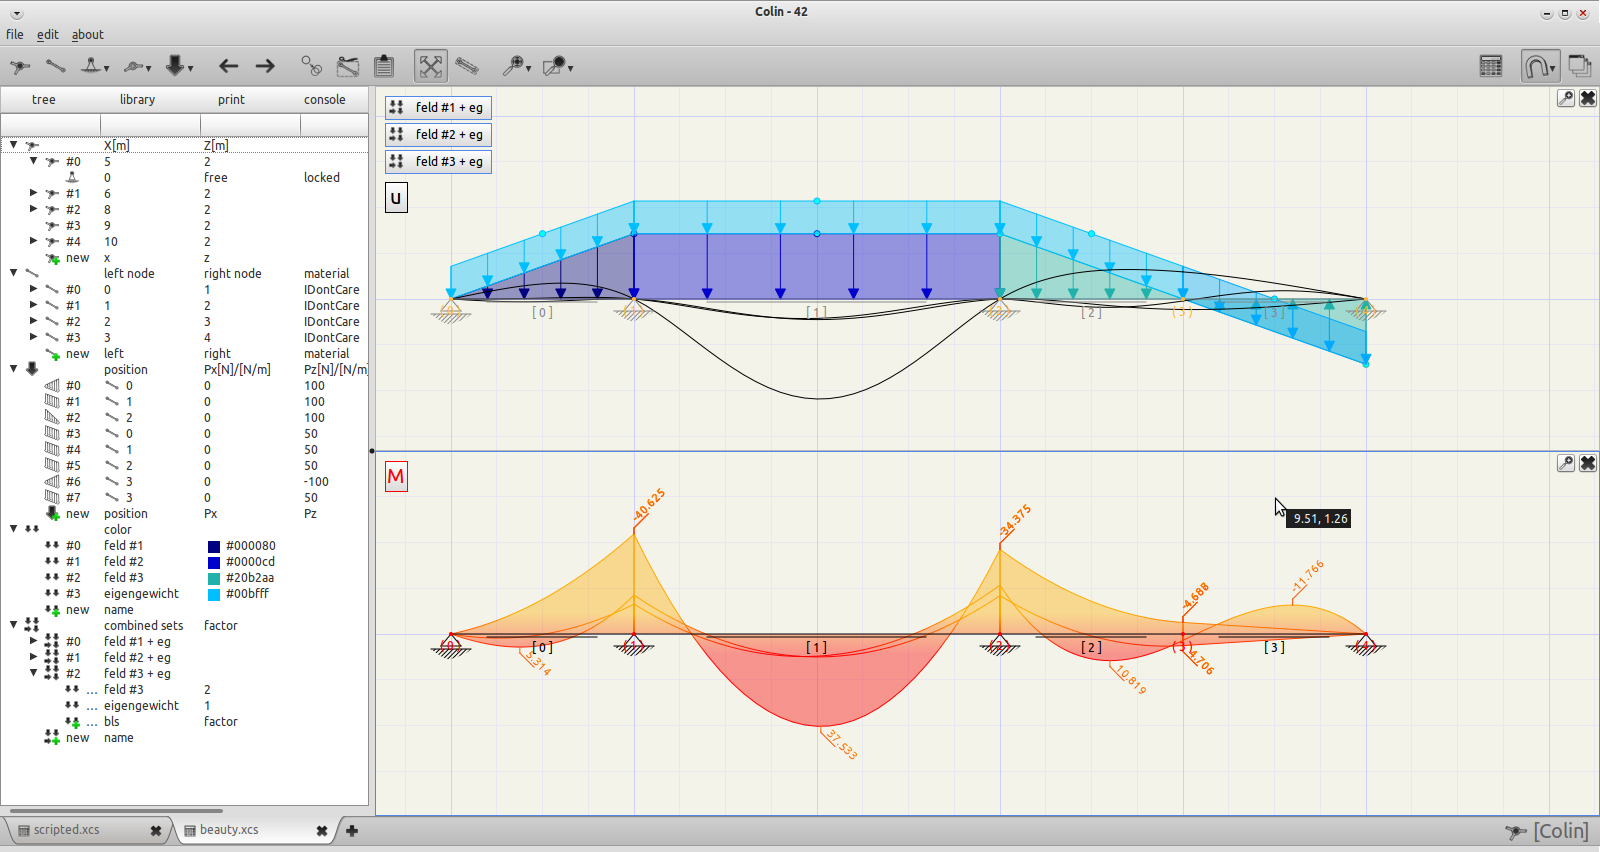
\includegraphics[width=\textwidth]{../pictures/title.png}
\end{center}
\vspace{40pt}
\begin{center}
\large{an open source structural analysis application}
\end{center}

\end{titlepage}
\clearpage


\begin{minipage}[h]{0.25\textwidth}
\begin{center}

\includegraphics[height=3cm]{./pictures/clazzes2.jpg}
\end{center}
\end{minipage}
\begin{minipage}[h]{0.75\textwidth}
\textbf{\large{Colin is a Clazzes.org Project.}}
\vspace{8pt}\\
www.clazzes.org
\end{minipage}
\vspace{20pt}
\hline
\vspace{20pt}
\begin{minipage}[h]{0.25\textwidth}
\begin{center}

\includegraphics[height=3cm]{./pictures/qt_ambassador_logo.png}
\end{center}
\end{minipage}
\begin{minipage}[h]{0.75\textwidth}
%\begin{flushright}
\textbf{\large{Colin is Part of the Qt Ambassador Programm.}}
\vspace{8pt}\\
qt.nokia.com/qtambassador
%\end{flushright}
\end{minipage}
\vspace{20pt}
\hline
\vspace{20pt}
\begin{minipage}[h]{0.25\textwidth}
\begin{center}

\includegraphics[height=3cm]{./pictures/logo2-icon_128x128.png}
\end{center}
\end{minipage}
\begin{minipage}[h]{0.75\textwidth}
%\begin{flushright}
\textbf{\large{With support and help from ITEG IT-Engineers}}
\vspace{8pt}\\
www.iteg.at
%\end{flushright}
\end{minipage}
\ \\

\vspace{250pt}


\begin{center}
	
\includegraphics[scale=0.5]{./pictures/280px-CreativeCommond_logo_trademark.png}
	
\includegraphics[scale=0.5]{./pictures/64px-Cc-by_new.png}
	
\includegraphics[scale=0.5]{./pictures/64px-Cc-sa_white.png}
\end{center}
\begin{center}This work is licensed under a Creative Commons Attribution-ShareAlike 3.0 License.\end{center}




\clearpage
\ \\
\vspace{470pt}
\ \\
Copyright \copyright 2011 Matthias Rauter(\href{mailto:matthias.rauter@student.uibk.ac.at}{matthias.rauter@student.uibk.ac.at})\\
\vspace{20pt} \ \\
\Colin is free software; you can redistribute it and/or modify it under the terms of the GNU General Public License as published by the Free Software Foundation; either version 3 of the License, or (at your option) any later version.\\
\Colin is distributed in the hope that it will be useful, but \textbf{without any warranty}; without even the implied warranty of \textbf{merchantability} or \textbf{fitness for a particular purpose}. See the GNU General Public License for more details.\\
You should have received a copy of the GNU General Public License along with this program; if not, see \url{http://www.gnu.org/licenses/}.


\clearpage

\tableofcontents
\listoffigures


\clearpage
\pagenumbering{arabic}

\chapter{What's Colin?}
\label{cha:colin}

\Colin is an structural analysis application. It's availible under the term of the GNU General Public License\footnote{\url{http://www.gnu.org/licenses/}}. Unlike most other licenses, the GNU GPL offers you the following:
\begin{enumerate}
	\item [0] the freedom to use the software for any purpose,
	\item [1] the freedom to change the software to suit your needs,
	\item [2] the freedom to share the software with your friends and neighbors, and
	\item [3] the freedom to share the changes you make.
\end{enumerate}\\
The source code of \Colin is availible at clazzes.org. Feel free to explore our SVN\footnote{\url{http://subversion.tigris.org/}} repository at \url{http://svn.clazzes.org/svn/colin/}. Prebuild packages are available for Debian GNU/Linux and Windows. Users of other operation systems can compile it themselves.\\

\Colin is limited to two dimensional structures and an analytical, linear analysis of those. Structures can be statically indeterminate. The following elements can be used to describe the physical structure:
\begin{itemize}
	\item \textit{Nodes} and \textit{Beams} to describe the geometry and physical properties
	\item \textit{Supports}, including springs and rotated supports
	\item \textit{Hinges} of all kind, including springs
	\item \textit{Loads}, including Nodal loads, linear distributed loads, temperature loads
	\item \textit{Basic Load Sets} and \textit{Combined Load Sets}
\end{itemize}\\
Besides, \Colin offers the following additional features for an easy handling:
\begin{itemize}
	\item complete CAD environment
	\item object, grid and orthogonal snap
	\item saving to XML
	\item unlimited undo/redo
	\item copy'n`paste
	\item printing
	\item table like editing in a tree representation
	\item JavaScript Engine including a console
\end{itemize}

I started coding Colin with the aim to create an application which can be used imeadetly after installation. Some advanced features as meterials and cross sections (unused when calculating statically determinated structrues as done a long period at our university), springs as supports or rotated supports, load sets, etc. can be ignored completly and should not disturb.\\
Of course this means also Colin does not contain any stupid, crapy, bullshit-register-here-activate-there-digital-rights-managment\footnote{\url{http://www.defectivebydesign.org/}}. 


\section{getting started on Linux}
\label{sec:startLinux}

If you use a Debian GNU/Linux based distribution, you can use our Debian repository. Debian GNU/Linux based distributions use the *.deb format to install packages. Debian, Ubuntu and Linux Mint should work with our packages. For distribution witch use *.rpm packages see section~\ref{sec:startOther}.\\

First you need to trust our archiver key. You can do so by opening a terminal and typing:
\begin{lstlisting}[frame=single, breaklines=true, basicstyle=\small]
wget https://www.clazzes.org/gpg/pba-archiver.clazzes.org.asc -O - | sudo apt-key add - 
\end{lstlisting}
Then you can add our repository to the software sources. To do so, open the \textit{Software Center}. To edit your software sources there, open the \textit{Edit} menu in the menubar and click on \textit{Software  Sources...} there.\\
A new Window should appear. Activate the \textit{Other Software} tab there. Click \textit{Add...} there and enter the following text, depending on your operation systems version:

\begin{itemize}
	\item Ubuntu Lucid Lynx 10.04 or newer and the corresponding Linux Mint
\begin{lstlisting}[frame=single, breaklines=true, basicstyle=\small]
deb http://deb.clazzes.org/ubuntu lucid-colin-1 main  
\end{lstlisting}
	\item Debian Squeeze 6
\begin{lstlisting}[frame=single, breaklines=true, basicstyle=\small]
deb http://deb.clazzes.org/debian squeeze-colin-1 main
\end{lstlisting}
\end{itemize}

After updating \textit{apt-get} you should be able to install \Colin.



\section{getting started on Windows}
\label{sec:startWindows}

You can find Windows Setups in our download area at clazzes.org: \url{http://download.clazzes.org/colin/testing/}. *x64* marks the 64 bit version, *x86* the 32 bit version. Download the right version for your Windows. You can install it by executing the Setup. \\

\textbf{note:}
\begin{center}
\textbf{Other than on Linux, the Windows version of \Colin does not get updated automatically. Please take look at clazzes.org from time to time to watch out for newer versions of \Colin. Or simply switch to Linux ;)}
\end{center}

\section{getting started on other OS}
\label{sec:startOther}

If you are using an OS for witch no packages are provided, you can download the source from our SVN repository and compile it your self. \Colin should work on most operation systems, including all UNIX like operation systems and OS X. To get \Colin compiled take a look at chapter~\ref{cha:compile}.\\
A version for OS/2 has already been compiled by some else. You can find it at ecomstation.it\footnote{\url{http://www.ecomstation.it/ecsoft2/prog.php?progid=1795&name=Colin&sys=os2+ecomstation}}. Please note that i don't keep this build up-to-date.


\chapter{Objects}
\label{cha:objects}

This chapter gives a quick overview over the objects in \Colin.

\section{Struct}
This object defines structures. It contains all Nodes, Beams, Loads, etc. 

\section{Node}
A Node defines the geometry of structures in \Colin. It contains the coordinates \textit{x} and \textit{z}. Supports can be added to Nodes.

\section{Support}
Supports define the boundary conditions of nodes. Use these to lock the displacement of nodes.

\section{Beam}
These objects represent the beams of the structure. They are spanned between two nodes. Beams contain a reference to their left and right node, their cross section and their material. Besides, hinges can be assigned to beams to define boundary conditions.

\section{Hinge}
Hinges define boundary conditions of beams. 

\section{Loads}
These objects define the load on the structure.

\subsection{Nodal Load}
A simple load on a node.

\subsection{Moment}
A moment on a node.

\subsection{Distributed Loads}
Linear distributed or uniformly distributed loads on beams.

\subsection{Temeperatur Loads}
Loads due to temperature changes or temperature differences.
 
\subsection{Double Load} 
Loads between the left and right side of a hinge.

\section{Basic Load Set}
Loads can be assigned to Basic Load Sets (BLS) to group them.

\section{Combined Load Set}
Combine groups of loads for the calculation of many cases in once.

\section{Material}
The material defines material properties of beams, \textit{stiffness} E and \textit{thermal expansion coefficient} $\alpha_T$.

\section{Cross Section}
Cross Sections define the geometry of beams in their local y-z plane,  \textit{height} h, \textit{area} A and \textit{second moment of area} I.

\chapter{Graphical User Interface}

This chapter gives an overview over the Graphical User Interface (GUI) of Colin.

\section{Workspace}
\label{sec:workspace}

Here a quick overview over the Workspace. This is the part of the GUI you are actually working with. The different parts are explained in depth later.
\begin{figure}[H]
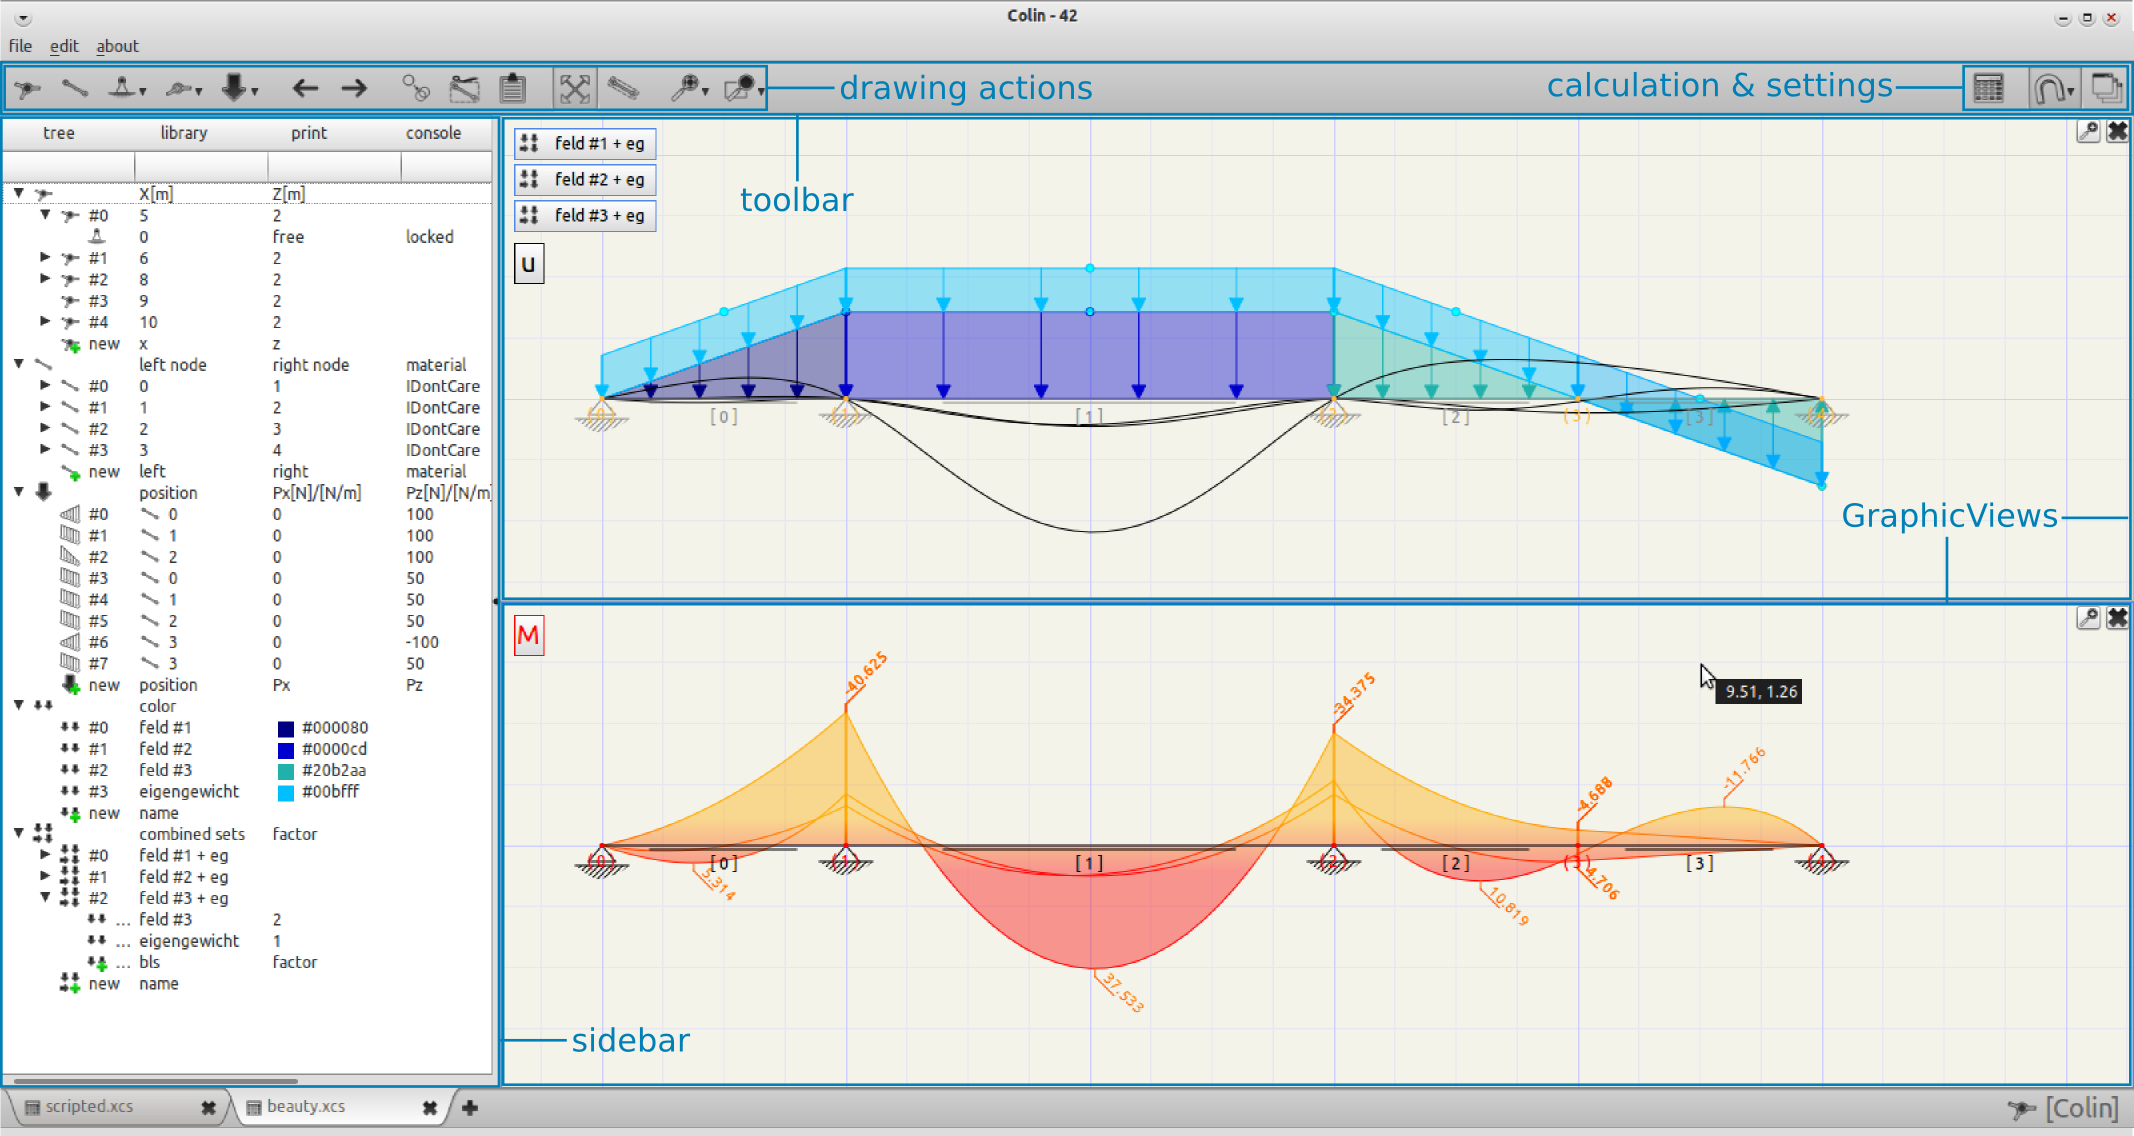
\includegraphics[width=\textwidth]{../pictures/workspace_overlay.png}
\caption{Workspace}
\label{pic:workspace}
\end{figure}

Figure~\ref{pic:workspace} shows the elements of the workspace:
\begin{itemize}
	\item Menubar: On the top of the Mainwindow. See section~\ref{sec:menubar}.
	\item Toolbar: 
	\begin{itemize}
		\item drawing actions: these actions interact with the GraphicsView
		\item calculation and settings: here you can find some quick settings for the snap and the shown windows. also the action to calculate forces of the structure is placed here.
	\end{itemize}
	See section~\ref{sec:toolbar}.
	\item Sidebar: the sidebar contains additional views and widgets:
	\begin{itemize}
		\item tree: shows a tree which represents the current structure. See section~\ref{ssec:tree}.
		\item library: gives access to the library (stored materials and cross sections). See section~\ref{ssec:library}.
		\item print: shows a printing dialog. See section~\ref{ssec:printingwidget}.
		\item console: a console which interprets Javascript and  See section~\ref{ssec:console}.
	\end{itemize}
	See section~\ref{sec:sidebar}.
	\item GraphicsView: Here you can see the graphical representation of a structure and the results of the calculation. Also, you can draw new elements and manipulate existing ones. See section~\ref{sec:graphical}.
	\item Tabbar: Shows the opened files. See section~\ref{sec:tabbar}.
\end{itemize}

\section{Menubar}
\label{sec:menubar}
The menubar is placed on top of the Mainwindow on most operation systems. The \textit{file} menu contains some basic actions to organize, such as \textit{open} and \textit{save} (see figure~\ref{pic:filemenu}). The \textit{edit} menu contains some additional actions to manipulate the current file (see figure~\ref{pic:editmenu}) which are not present in the toolbar (see section~\ref{sec:toolbar}. You can activate these action by pressing the shortcut. It's visible next to the corresponding action.

\begin{minipage}[b]{\textwidth/2}
\begin{figure}[H]
\begin{center}
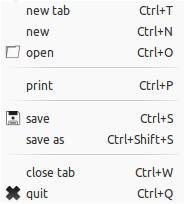
\includegraphics[scale=0.6]{../pictures/filemenu.png}
\caption{menu: \textit{file}}
\label{pic:filemenu}
\end{center}
\end{figure}
\end{minipage}
\begin{minipage}[b]{\textwidth/2}
\begin{figure}[H]
\begin{center}
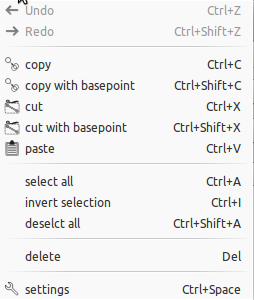
\includegraphics[scale=0.6]{../pictures/editmenu.png}
\caption{menu: \textit{edit}}
\label{pic:editmenu}
\end{center}
\end{figure}
\end{minipage}


\subsection{file menu}
Here a quick overview over the action present in this menu:
\begin{itemize}
	\item \textit{new tab}: shows the start page
	\item \textit{new}: creates a new empty file
	\item \textit{open}: open a file on your computer
	\item \textit{print}: launches the print dialog
	\item \textit{save}: saves the current file. Overwrites any other version. If the file was not saved before, a dialog appears where you can enter the designated filename
	\item \textit{save as}: saves the current file. Asks for a filename.
	\item \textit{close tab}: closes the current tab. Asks for saving the file has been edited.
	\item \textit{quit}: closes the application. Asks for saving before.
\end{itemize}

\subsection{edit menu}
A quick overview over the \textit{edit} menu. 
\begin{itemize}
	\item \textit{Undo}: undo the last change.
	\item \textit{Redo}: redo the last undone change.
	\item \textit{copy}: copy all currently selected objects to the clipboard. 
	\item \textit{copy with basepoint}: like copy, but when pasting form clipboard, you can chose the position where it gets inserted in relation to the given basepoint. More in section~\ref{sec:graphical}.
	\item \textit{cut}: like copy, deletes original objects.
	\item \textit{cut with basepoint}: like copy with basepoint, deletes original objects.
	\item \textit{paste}: paste from clipboard.
	\item \textit{select all}: selects all elements of the current structures.
	\item \textit{invert selection}: selects all elements of the current structure which are not selected and vise versa.
	\item \textit{deselect all}: removes selection state from all objects.
	\item \textit{delete}: deletes the currently selected objects.
	\item \textit{settings}: launces the settings page.
\end{itemize}
\section{Tabbar}
\label{sec:tabbar}
This bar can be found on the buttom of the Colin GUI. You can see all open files and active them by clicking on them. Press the cross to close a tab. Press "+" to open a new tab.
\begin{figure}[H]

\includegraphics[width=\textwidth]{../pictures/tabbar.png}
\caption{tabbar}
\label{pic:tabbar}
\end{figure}

\section{Toolbar}
\label{sec:toolbar}

The toolbar contains the most used actions. Icons with a triangle besides them are expandable. You can trigger a menu with more options by keeping the button pressed long. When moving the mouse over a icon a tooltip with some basic informations of the usage appears. 

\begin{figure}[H]

\includegraphics[width=\textwidth]{../pictures/toolbar.png}
\caption{toolbar}
\label{pic:toolbar}
\end{figure}

Here the actions in the toolbar from left to right.
\subsection{Nodes}
When activated, you can draw Nodes by clicking on the designated position in the GraphicsView. When you click on a beam, the beam gets spitted at the clicked position, when clicking on 2 crossing beams, the get both splitted and connected with a new node.

\subsection{Beams}
When activated, you can draw Beams, by clicking on the designated nodes in the GraphicView. If you do not click on a node, a new node will be created. Material and cross section are chosen automatically. You can set the material and cross section of beams created like this in the library widget (see section~\ref{ssec:library}). You can edit them afterwards too. This is shown in section~\ref{sec:graphical} (by using the GraphicView) and in section~\ref{ssec:tree} (by using the tree representation).

\subsection{Supports}
\begin{minipage}[h]{4cm}
\begin{figure}[H]
\begin{center}
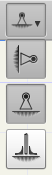
\includegraphics[scale=0.6]{../pictures/support_opt.png}
\caption{options}
\label{pic:support_opt}
\end{center}
\end{figure}
\end{minipage}
\begin{minipage}[h]{\textwidth-4cm}
When activated, you can add supports to nodes by clicking on the in the GraphicsView. Keep the mouse button pressed to get access to more settings. The buttons as shown in figure~\ref{pic:support_opt} appear. Here you can set the basic form of the support which gets added to a nodes by clicking on them:
\begin{trivlist}
	\item[] 
\includegraphics[scale = 0.5]{../../icons/bearingH.png} horizontal support: the horizontal displacement will be zero
	\item[] 
\includegraphics[scale = 0.5]{../../icons/bearing.png} vertical support: the vertical displacement of the node will be zero
	\item[] 
\includegraphics[scale = 0.5]{../../icons/bearingM.png} rotational support: the rotation of the node will be zero
\end{trivlist}
You can choose any combination of these 3 basic supports. To use springs as supports and for rotated supports see section~\ref{ssec:tree}.
\end{minipage}

\subsection{Hinges}

\begin{minipage}[h]{4cm}
\begin{figure}[H]
\begin{center}
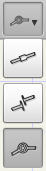
\includegraphics[scale=0.6]{../pictures/hinge_opt.png}
\caption{options}
\label{pic:hinge_opt}
\end{center}
\end{figure}
\end{minipage}
\begin{minipage}[h]{\textwidth-4cm}
When activated, you can add hinges to beams. Click on a beam to add a hinge at the designated position of the beam. Click near the left or right node of a beam to put the hinge to the right or left end of the beam. Keep the button pressed to get access to more settings. You can choose the the type of hinge by clicking on the respective button:
\begin{trivlist}
	\item[] 
\includegraphics[scale = 0.5]{../../icons/jointN.png} normal force on the respective position will be zero.
	\item[] 
\includegraphics[scale = 0.5]{../../icons/jointQ.png} shear force on the respective position will be zero.
	\item[] 
\includegraphics[scale = 0.5]{../../icons/joint.png} moment on the respective position will be zero.
\end{trivlist}
If you want a sprint between the left and right side of a hinge take a look in section~\ref{ssec:tree}.
\end{minipage}

\subsection{Loads}

\begin{minipage}[h]{4cm}
\begin{figure}[H]
\begin{center}

\includegraphics[scale=0.6]{../pictures/load_opt.png}
\caption{options}
\label{pic:load_opt}
\end{center}
\end{figure}
\end{minipage}
\begin{minipage}[h]{\textwidth-4cm}
When activated you can add loads to the structure. Most of the actions here need two clicks to create a load. Figure~\ref{pic:drawload} shows the two required clicks for an uniformly distributed load. Keep the button pressed to get access to more settings. The possible types of loads:
\begin{trivlist}
	\item[] 
\includegraphics[scale = 0.5]{../../icons/load.png} nodal lode. Click on a node in the GraphicsView to specify the position of the load. The second click sets the values $P_x$ and $P_z$ of the load and completes the input.
	\item[] 
\includegraphics[scale = 0.5]{../../icons/moment.png} moment. Click on a node in the GraphicsView to specify the position of the moment. The second click sets the value $M$ of the load and completes the input.
	\item[] 
\includegraphics[scale = 0.5]{../../icons/ustload.png} uniformly distributed load. Click on a beam to specify the position of the load. The second click sets the values $P_x$ and $P_z$ of the load and completes the input.
	\item[] 
\includegraphics[scale = 0.5]{../../icons/istload.png} increasing linear load. just like the uniformly distributed load.
	\item[] 
\includegraphics[scale = 0.5]{../../icons/dstload.png} decreasing linear load. just like the uniformly distributed load.
	\item[] 
\includegraphics[scale = 0.5]{../../icons/temp.png} temperature load. Click on a beam to specify the designated position of the temperature load. The widget as shown in figure~\ref{pic:tempwidget} in form of a thermometer appears. You can switch between temperature change and temperature difference (between top and bottom of the cross section) by clicking the button besides the thermometer or pressing the left and right keys ($\leftarrow$ and $\rightarrow$) on your keyboard. You can set the temperature difference by clicking on the thermometer (the scale is adapted automatically) or with the up and down keys ($\uparrow$ and $\downarrow$) of your keyboard. \textbf{Complete the input with the \textit{Enter} key.}
	\item[] 
\includegraphics[scale = 0.5]{../../icons/doubleL.png} double loads between the left and right side of a hinge.
\end{trivlist}
\end{minipage}

\begin{minipage}[b]{\textwidth/2}
\begin{figure}[H]
\begin{center}
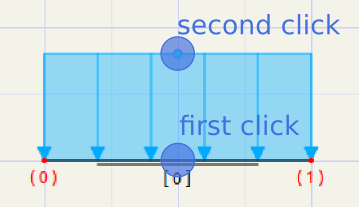
\includegraphics[height=3cm]{../pictures/drawload_overlay.png}
\caption{the two required clicks to draw a load}
\label{pic:drawload}
\end{center}
\end{figure}
\end{minipage}
\begin{minipage}[b]{\textwidth/2}
\begin{figure}[H]
\begin{center}
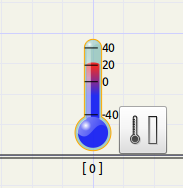
\includegraphics[height=3cm]{../pictures/temp_wid.png}
\caption{adding a temperature load}
\label{pic:tempwidget}
\end{center}
\end{figure}
\end{minipage}

\subsection{Undo/Redo}
\begin{minipage}[h]{4cm}
\begin{figure}[H]
\begin{center}

\includegraphics[scale=0.6]{../pictures/undoredotoolbar.png}
\caption{Undo}
\label{pic:undoredotoolbar}
\end{center}
\end{figure}
\end{minipage}
\begin{minipage}[h]{\textwidth-4cm}
\begin{trivlist}
	\item[] 
\includegraphics[scale = 0.5]{../../icons/undo.png} Undo: to revert the last modification of the current file.
	\item[] 
\includegraphics[scale = 0.5]{../../icons/redo.png} Redo: to repeat the last undone modification.
\end{trivlist}
\end{minipage}

\subsection{Copy/Cut/Paste}
\begin{minipage}[h]{4cm}
\begin{figure}[H]
\begin{center}

\includegraphics[scale=0.6]{../pictures/clipboardtoolbar.png}
\caption{Clipboard}
\label{pic:clipboardtoolbar}
\end{center}
\end{figure}
\end{minipage}
\begin{minipage}[h]{\textwidth-4cm}
\begin{trivlist}
	\item[] 
\includegraphics[scale = 0.5]{../../icons/copy.png} Copy: copy the currently selected objects to the clipboard.
	\item[] 
\includegraphics[scale = 0.5]{../../icons/cut.png} Cut: copy the currently selected objects to the clipboard and delete the selection afterwards.
	\item[] 
\includegraphics[scale = 0.5]{../../icons/paste.png} Paste: paste the objects in the clipboard. You need to enter a basepoint in the Graphicsview to complete the procedure. 
\end{trivlist}
\end{minipage}

\subsection{Move}

\begin{minipage}[h]{4cm}
\begin{figure}[H]
\begin{center}

\includegraphics[scale=0.6]{../pictures/movetoolbar.png}
\caption{Move}
\label{pic:movetoolbar}
\end{center}
\end{figure}
\end{minipage}
\begin{minipage}[h]{\textwidth-4cm}
This is the Standard Action in Colin. You can active it with the \textit{Escape} key. When activated you can navigate easily thorough the GraphicViews (see section~\ref{sec:graphical} for a deeper view into navigation). 
You can also move/manipulate the most objects in GraphicView by click them and move the mouse while pressed the mouse button. For a deeper view into this mechanism take a look into section~\ref{sec:graphical}.
\end{minipage}

\subsection{Select}

\begin{minipage}[h]{4cm}
\begin{figure}[H]
\begin{center}

\includegraphics[scale=0.6]{../pictures/selecttoolbar.png}
\caption{Select}
\label{pic:selecttoolbar}
\end{center}
\end{figure}
\end{minipage}
\begin{minipage}[h]{\textwidth-4cm}
When activated you can select objects in the GraphicsView by clicking on them. The previous selection is unselected. To keep the previous selection, press \textit{Shift} while clicking.\\
You can also span a rectangle by clicking on a position in the GraphicView and keep the mouse pressed. Release the mouse button when the rectangle contains all object you want to select. See figure~\ref{pic:graphicalselectionrect} to get an idea. You can also select objects in the tree representation in the sidebar, independent form the active tool (see section~\ref{ssec:tree}).
\end{minipage}

\begin{figure}[H]
\begin{center}
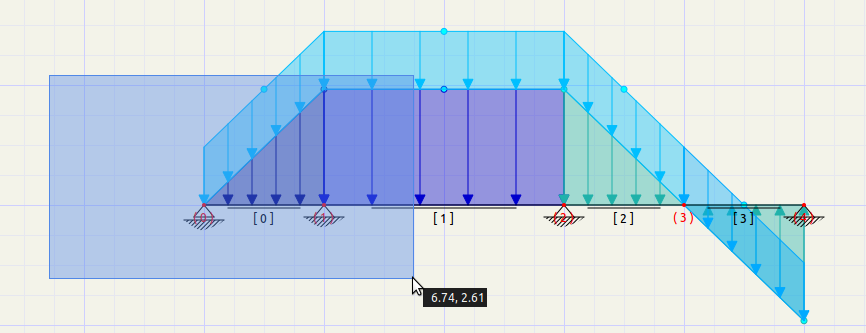
\includegraphics[width=\textwidth]{../pictures/selectionrect.png}
\caption{Selecting a Rect}
\label{pic:graphicalselectionrect}
\end{center}
\end{figure}


\subsection{Autozoom and scaling}
\begin{minipage}[h]{7cm}
\begin{figure}[H]
\begin{center}
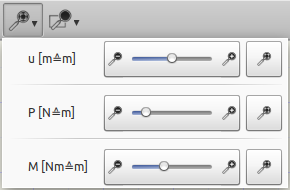
\includegraphics[scale=0.6]{../pictures/scaletoolbar.png}
\caption{Scaling menu}
\label{pic:scaletoolbar}
\end{center}
\end{figure}
\end{minipage}
\begin{minipage}[h]{\textwidth-7cm}
A short click on this button activates the auto zoom. The GraphicViews are adjusted so that the current structure fits well into them.\\
Keep the mouse button pressed to get access to the menu shown in figure~\ref{pic:scaletoolbar}. You see a slider for the scaling of the deformation, a slider for forces and a slider for moments. The slider can be used to adjust the scaling of these in the GraphicsViews. The magnifying glasses left and right from the slider can be pressed to adjust the scaling too. The buttons on the right side of the menu active the autozoom for the corresponding physical values. You can also adjust zoom with the mouse wheel and the mouse wheel in combination with some modifiers. See section~\ref{sec:graphical} and section~\ref{ssec:miscsettings} for more information about the zooming with the mousewheel.
\end{minipage}

\subsection{Zoom}

\begin{minipage}[h]{4cm}
\begin{figure}[H]
\begin{center}

\includegraphics[scale=0.6]{../pictures/zoom_opt.png}
\caption{Options}
\label{pic:zoom_opt}
\end{center}
\end{figure}
\end{minipage}
\begin{minipage}[h]{\textwidth-4cm}
The zoom tool can be used to adjust the general scaling of the GraphicViews. Keep the mouse button pressed to get access to more zooming tools:
\begin{trivlist}
	\item[] 
\includegraphics[scale = 0.5]{../../icons/zoom_rect.png} Zoom Rectange: When this tool is selected you can specify a rectangle in the GraphicsView as in figure~\ref{pic:graphicalselectionrect}. The scale will be adjusted so that the selected rectangle fits into the view.
	\item[] 
\includegraphics[scale = 0.5]{../../icons/zoom_in.png} Zoom in: Click on the Graphicsview to zoom in.
	\item[] 
\includegraphics[scale = 0.5]{../../icons/zoom_out.png} Zoom out: Click on the Graphicsview to zoom out.
\end{trivlist}
\end{minipage}

\subsection{Calculate}

\begin{minipage}[h]{4cm}
\begin{figure}[H]
\begin{center}

\includegraphics[scale=0.6]{../pictures/calctoolbar.png}
\caption{Calculate}
\label{pic:calctoolbar}
\end{center}
\end{figure}
\end{minipage}
\begin{minipage}[h]{\textwidth-4cm}
Press to calculate the forces in the structure. When the calation has failed or finished successfully, a widget appears under this button. It contains informations about the calculation.
\end{minipage}

\subsection{Snap}

\begin{minipage}[h]{4cm}
\begin{figure}[H]
\begin{center}
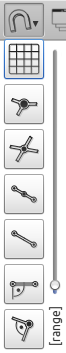
\includegraphics[scale=0.6]{../pictures/snap_opt.png}
\caption{Options}
\label{pic:snap_opt}
\end{center}
\end{figure}
\end{minipage}
\begin{minipage}[h]{\textwidth-4cm}
This button offers some options for the snap function of the GraphicsView (see section~\ref{sec:graphical}). You should know snap from other CAD applications. The snap tool can be enabled or disabled with a short click. For some actions, for which the snap function is required as adding supports or loads to the structure, the snap is always active. Keep the mouse button pressed to get access to more options. You can enable and disable specific snap functions by clicking on the related button.
\begin{trivlist}
	\item[] 
\includegraphics[scale = 0.5]{../../icons/grid.png} Grid: If near the grid, the mouse gets snaped an moved to the grid. Also, when drawing a load or a beam with actived grid snap, the snap helps to enter beams with rounded lengths and rounded loads.
	\item[] 
\includegraphics[scale = 0.5]{../../icons/node.png} Node: Snap nodes while drawing beams. This option must be on to connect existing nodes. When turned of, a click near a node will create a new node.
	\item[] 
\includegraphics[scale = 0.5]{../../icons/crossing.png}Intersecting beams: When active, you will be able to snap the intersection of two beams. This allows to draw nodes in the position where the beams are intersecting. The intersecting beams will be connected to the new node when you do so.
	\item[] \includegraphics[scale = 0.5]{../../icons/middle.png} Middle of beams: When active, the snap helps you to split beams in two sections with the same length while drawing nodes or beams. Also node loads can be put on beams (a new node is created automatically). With this option the middle of a beam is prefered.
	\item[] \includegraphics[scale = 0.5]{../../icons/beam.png} Beams: While drawing nodes or beams, positions on beams are prefered. The beam snaped is connected to created nodes.
	\item[] \includegraphics[scale = 0.5]{../../icons/ortho_g.png} Global orthogonal: When enabled, the snap helps you to draw horizontal and vertical beams and loads.
	\item[] \includegraphics[scale = 0.5]{../../icons/ortho_l.png} Local orthogonal: When activated, the snap helps you to draw beams normal or parallel to existing beams. While drawing loads, the snap helps you to draw loads normal or parallel to the beam where the load is put on.
	\item[] \textbf{[range]}: The slider on the right side of the buttons can be used to adjust the range which the snap interprets as "near".
\end{trivlist}
\end{minipage}


\subsection{Windows}

\begin{minipage}[h]{7cm}
\begin{figure}[H]
\begin{center}
\includegraphics[scale=0.6]{../pictures/windowtoolbar.png}
\caption{Window menu}
\label{pic:windowtoolbar}
\end{center}
\end{figure}
\begin{figure}[H]
\begin{center}
\includegraphics[scale=0.6]{../pictures/windowtoolbar2.png}
\caption{Select GraphicViews}
\label{pic:windowtoolbar2}
\end{center}
\end{figure}
\end{minipage}
\begin{minipage}[h]{\textwidth-7cm}
After a click on the window tool button the menu in figure~\ref{pic:windowtoolbar} appears. You can see three menu entrys:
\begin{itemize}
	\item \textit{fullscreen}: Switch fullscreen mode on and off.
	\item \textit{show all}: Show all GraphicViews.
	\item \textit{show sidebar}: Hide and show the sidebar.
\end{itemize}
The four rectangles in this menu can be used to chose the visilbe GraphicViews. The GraphicViews are explaned in depth in section~\ref{sec:graphical}. You can click on a single rectangle to show the related GraphicsView. The currently visilbe GraphicViews are highlighted as the GraphicsView on the button left in figure~\ref{pic:windowtoolbar2}. The notations whitin the rectangles shows the data visulized in the related GraphicsView. You can also select more of them as shown in figure~\ref{pic:windowtoolbar2}. To do so, click on a Point in the area. A rectangle appears. Keep the mouse pressed and move the mouse until the rectanlge covers all GraphicViews you want to be shown. After releasing the mousebutton, a selection as in figure~\ref{pic:windowtoolbar2} would show the two GraphicsViews on the top. 
\end{minipage}


\section{GraphicView}
\label{sec:graphical}

Some text!!!!


\subsection{Right Click Widgets}
\label{sec:rightclickwidgets}

A right click will show you a widget with more information about the item clicked. Depending on the item clicked, one of the following widgets will appear:
\begin{trivlist}
	\leftskip=1cm
	\item[] \includegraphics[scale = 0.5]{../../icons/grid.png} \textbf{background}: A widget for overall inforamtion, see section~\ref{sec:nodedetail}.
	\item[] \includegraphics[scale = 0.5]{../../icons/node.png} \textbf{nodes}: The widget for nodes, see section~\ref{sec:nodedetail}.
	\item[] \includegraphics[scale = 0.5]{../../icons/beam.png} \textbf{beams}: The widget for beams, see section~\ref{sec:nodedetail}.
	\item[] \includegraphics[scale = 0.5]{../../icons/load.png} \textbf{loads}: The widget for loadss, see section~\ref{sec:nodedetail}.
	
\end{trivlist}



These widgets are all organised in toolboxes. You can hide and show most of the toolboxes of these widgets by clicking on the corresponding checkbox in the top right of the toolbox. Some very important sections will always be shown and are not hideable.\\
All widgets can be closed pressing the \textif{Escape} key or pressing the red cross in the upper right corner of the widget. \\
Those widgets, which are related to a specific element of the structure, contain 3 buttons as shown in figure~\ref{pic:overlayheader}. Press "\textit{<}" or "\textit{>}" to switch to another element (of the same type). The number and icon in the middle marks the currently shown item.

\begin{figure}[H]
\begin{center}
\includegraphics[width=\textwidth]{../pictures/overlayheader.png}
\caption{header item of a right click widget}
\label{pic:overlayheader}
\end{center}
\end{figure}


\subsection{Structure proerties}
\label{sec:structdetail}


\begin{figure}[H]
\centering{
\includegraphics[width=\textwidth]{../pictures/generaloverlay.png}
\caption{structure properties}
}
\label{pic:generaloverlay}
\end{figure}

This view appears after a \textbf{right click} on the background of the view widget. It shows some basic overall information. 

\paragraph{paste}
This element (placed on the left side of the screen, see also figure~\ref{pic:generaloverlay}) shows an overview over all parts which have been copied by any instance of \Colin. This can be nodes (with the corresponding support), beams (with the corresponding nodes and their properties), loads (including their basic load set) or many items. You can remove them from the temporary memory by clicking on the red cross in the upper right corner of the preview. You can insert them to your current file by clicking on the preview. This view will disappear immediately to allow you to specify the position where the copied elements should be insert. Click on the designated position to finish the procedure. The copied parts are now part of your current file. 

\paragraph{export}
This element (placed in the middle of the screen, see also figure~\ref{pic:generaloverlay}) allows you to export a picture of your current view on the structure. The picture contains the same elements and functions as the view you picked to launch this menu. The zoomfactor of all loads and functions matches also to those in the viewports.
The picture on top shows a preview of the exported file. Below, you can set some properties to make sure the picture matched to your needs:
\begin{trivlist}
	\leftskip=1cm
	\item[]\textbf{left}: The left boundary of the rectangle which is exported in global coordinates (meters).
	\item[]\textbf{right}: The right boundary of the rectangle which is exported in global coordinates (meters).
	\item[]\textbf{top}: The top boundary of the rectangle which is exported in global coordinates (meters).
	\item[]\textbf{botton}: The top boundary of the rectangle which is exported in global coordinates (meters).
	\item[]\textbf{resolution (x)}: The horizontal resolution of the resulting image in pixel
	\item[]\textbf{resolution (z)}: The vertical resolution of the resulting image in pixel
	\item[]\textbf{scale text}: Used to scale up or down text and elements or symbols with a fixed pixel size, such as supports and hinges.
\end{trivlist}

\paragraph{combined load sets}
Shows the combined load sets this structure contains.

\paragraph{basic load sets}
Shows the basic load sets this structure contains.

\subsection{Detail/Edit View for nodes}
\label{sec:nodedetail}



\begin{figure}[H]
\centering{
\includegraphics[width=\textwidth]{../pictures/nodeoverlay.png}
\caption{structure properties}
\label{pic:generaloverlay}
}
\end{figure}

This view appears after a \textbf{right click} on a node. It shows all properties of the node and allows edition (left row). Also, this view offers a detailed view to results for this node (center and right row).

\paragraph{coordinates}
Set the coordinates of the node:
\begin{trivlist}
	\leftskip=1cm
	\item[]\textbf{x}: horizontal coordinate of the node in meters
	\item[]\textbf{z}: vertical coordinate of the node in meters
	\item[]\textbf{phi}: the angle of the local coordinate system of the node. Editing is disabled if no support is set for this node. The local coordinate system affects only nodes with supports. Counterclockwise angles are positive!
\end{trivlist}

\paragraph{support}
The first three buttons allow to set the support for this note:
\begin{trivlist}
	\leftskip=1cm
	\item[]\includegraphics[scale = 0.5]{../../icons/bearingH.png} Horizontal support: toggle to set/remove
	\item[]\includegraphics[scale = 0.5]{../../icons/bearingV.png} Vertical support: toggle to set/remove
	\item[]\includegraphics[scale = 0.5]{../../icons/bearingM.png} Moment support: toggle to set/remove
\end{trivlist}





\begin{minipage}[h]{6.5cm}
\begin{figure}[H]
\begin{center}
\includegraphics[width=6cm]{../pictures/supportextended.png}
\caption{setting springs}
\label{pic:supportextended}
\end{center}
\end{figure}
\end{minipage}
\begin{minipage}[h]{\textwidth-7cm}
You can also set springs by checking the \textif{springs} ckeckbox. An extended toolbox as in figure~\ref{pic:supportextended} appears. To add a spring to your node, press the \includegraphics[scale=0.5]{../../icons/spring.png} button next to the designated direction. The textbox next to the button will be activated and allow entering of a spring constant. The unit is shown at the end of the row (it can be set in the settings part, see also section~\ref{ssec:miscsettings}) 
\end{minipage}


\paragraph{clipboard}
Use the \includegraphics[scale=0.5]{../../icons/spring.png} \textit{copy} or \includegraphics[scale=0.5]{../../icons/spring.png} \textit{cut} button to copy the current node to the clipboard. The support gets copied too. Therefore, this feature can be used to assign supports very quickly to your nodes.

\paragraph{view}
Shows a detailed view on the current node. Colors are the same as in the viewport. Beside reaction forces, the graphic shows all forces in beams connected to this node. If you are using load set and combined load sets, the same CLS as in the viewport are shown here.

\paragraph{displacement}
Shows the displacement of the node. If you are using load sets and the value is the zero for all load sets, only one value is shown (labeled with $_{\max}$). Otherwise, all values are shown, below the maximum absolute value (labeled with $_{\max}$).
\textbf{You can select this text and copy it to your clipboard!} The index in the notation is the index of the CLS which leads to the respective displacement (for example, $u_{\max} = \text{absolute maximum of horizontal displacement}$, $u_{i} = \text{horizontal displacement of CLS i}$).

\paragraph{reactions}
Shows the reaction forces of the node. As for the displacement, the absolute maximum is shown on the top. Also, only one value is shown if all reaction forces of this direction are zero. They will not be listed if there is no support for the respective degree of freedom. Of course, this text can be copied to clipboard too.

\paragraph{beam forces}
Lists the forces in all beams connected to the note at the position where it is connected to the note. Only minimal and maximum value are shown if you are using CLS. Can also be copied.

\subsection{Detail/Edit View for beams}
\label{sec:beamdetail}



\begin{figure}[H]
\centering{
\includegraphics[width=\textwidth]{../pictures/beamoverlay.png}
\caption{structure properties}
\label{pic:beamoverlay}
}
\end{figure}

This view appears after a \textbf{right click} on a beam. It shows all properties of the beam and allows edition (left row). Also, this view offers a detailed view to results for this beam (center and right row).

\paragraph{nodes}
Here you can view and set the nodes which define the geometry of the beam:
\begin{trivlist}
	\leftskip=1cm
	\item[]\textbf{from}: The left node of the beam
	\item[]\textbf{to}: The right node of the beam
\end{trivlist}

\paragraph{geometry}
Shows additional geometry information, calculated by the application:
\begin{trivlist}
	\leftskip=1cm
	\item[]\textbf{alpha}: the angle between the beam and the global x axis. Counterclockwise angles are positive!
	\item[]\textbf{length}: the length of the beam
\end{trivlist}

\paragraph{hinges}
The two basic buttons allow to add ordinary hinges (setting the moment at the designated position to zero), left button for a hinge between left end of the beam and the left node, the right button for a hinge between right end of the bean and the right node.\\
\begin{minipage}[h]{6.5cm}
\begin{figure}[H]
\begin{center}
\includegraphics[width=6cm]{../pictures/hingesextended.png}
\caption{extended hinge options}
\label{pic:hingesextended}
\end{center}
\end{figure}
\end{minipage}
\begin{minipage}[h]{\textwidth-7cm}
You can toogle the \textit{more...} checkbox to get access to a much more features as shown in figure~\ref{pic:hingesextended}. In addition to the basic option, this toolbox offers the posibility to add hinges for all degree of freedoms and springs for all hinges! This toolbox contains six rows. Every row represents one degree of freedom in the following order: $u_l$, $w_l$, $\varphi_l$, $u_r$, $w_r$, $\varphi_r$. Springs can be set the same way as for supports (see section~\ref{sec:nodedetail}).
\end{minipage}


\paragraph{properties}
\begin{trivlist}
	\leftskip=1cm
	\item[]\textbf{material}: the material assigned to this beam
	\item[]\textbf{cross section}: the cross section assigned to this beam
\end{trivlist}

\paragraph{clipboard}
Use the \includegraphics[scale=0.5]{../../icons/spring.png} \textit{copy} or \includegraphics[scale=0.5]{../../icons/spring.png} \textit{cut} button to copy the current beam to the clipboard. Nodes and hinges related to this beam are copied too.



\begin{minipage}[h]{0.5\textwidth-0.5cm}
\begin{figure}[H]
\begin{center}
\includegraphics[width=\textwidth]{../pictures/externforcesdetail.png}
\caption{extern forces of the beam}
\label{pic:externforces}
\end{center}
\end{figure}
\end{minipage}
\hfill
\begin{minipage}[h]{0.5\textwidth-0.5cm}
\begin{figure}[H]
\begin{center}
\includegraphics[width=\textwidth]{../pictures/internforcesdetail.png}
\caption{intern forces of the beam}
\label{pic:internforces}
\end{center}
\end{figure}
\end{minipage}













\subsection{Detail/Edit View for loads}
\label{sec:loaddetail}

\section{Sidebar}
\label{sec:sidebar}

\subsection{Tree Representation}
\label{ssec:tree}


\begin{figure}
\centering{
\includegraphics[width=0.8\textwidth]{../pictures/tree.png}
\caption{tree widget}
}
\label{pic:tree}
\end{figure}


The tree representation allows a detailed view and editing of the current file. 

\paragraph{Navigation}
You can move throw the tree with the following keys (should be the same as in most spreadsheet applications):
\begin{trivlist}
	\leftskip=1cm
	\item[] \textbf{Tab}: next row or the first row in the next column if the end of the column was reached
	\item[] \textbf{Backtab}: previous row or the last row in the previous column if the beginning of the column was reached
	\item[] \textbf{Left}(arrow key): move backward within the current cell
	\item[] \textbf{Right}(arrow key): move forward within the current cell
	\item[] \textbf{Up}(arrow key): same property of the item above or the same property of the last item if the beginning of the row was reached
	\item[] \textbf{Down}(arrow key): same property of the item below or the same property of first item if the end of the row was reached
	\item[] \textbf{F2}: enter editing mode: opens an editor for the currently selected value
	\item[] \textbf{Enter}: Finish editing
	\item[] \textbf{Esc}: Abort editing
\end{trivlist}


All values can also be edited by clicking on them and entering the designated value.\\

\paragraph{Organization}

The tree contains 5 top level entries. All of them can be expanded to show their respective items. Some underlying entries can by expanded as well by clicking on the triangle on the left side.\\

Some entries are also marked with a green plus. This indicated that this entry can be used to add new items to the structure.


\begin{trivlist}
	\item[] \includegraphics[scale = 0.5]{../../icons/node.png} \textbf{nodes}: Contains all nodes. Each row shows one node, the last row shows a void entry which can be used to add nodes to the structure. A new node is added to the structure, when the coordinates have been set. All other properties can be set afterwards. Each column shows on the following properties:
	\begin{trivlist}
		\leftskip=1cm
		\item[]\textbf{x}: shows the x coordinate of the node
		\item[]\textbf{z}: shows the z coordinate of the node
		\item[]\textbf{phi}: shows the angle of the local coordinate system of the node. A node has only a local coordinate system if a support is set for the node.
	\end{trivlist}
	node entrys can be expanded to show: 
	\begin{trivlist}
		\leftskip=1cm
		\item[] \includegraphics[scale = 0.5]{../../icons/bearing.png} \textbf{supports}: Each column shows one of the following:
		\begin{trivlist}
		\leftskip=2cm
		\item[]\textbf{x}: shows the support of the node in x direction. This value can be \textit{free} or \textit{locked}. Also, you can add a numeric value to force \colin to add a spring as support to this node. The sprin constand will be the entered value.
		\item[]\textbf{z}: shows the support of the node in y direction. Same usage as for x direction.
		\item[]\textbf{phi}: shows the support of the node against rotation. Same usage as for x direction.
		\end{trivlist}
	\end{trivlist}
	\item[] \includegraphics[scale = 0.5]{../../icons/beam.png} \textbf{beams}: Contains all beams. Each row shows one beam, the last row shows a void entry which can be used to add beams. A new beam is added to the structure, when the nodes which define it's geometry have been set. All other properties can be set afterwards. Each column shows one of the following properties:
	\begin{trivlist}
		\leftskip=1cm		
		\item[]\textbf{from}: the left node of the beam
		\item[]\textbf{to}: the right node of the beam
		\item[]\textbf{material}: the material of the beam. Can be chosen in a list when clicking on the parameter
		\item[]\textbf{cross section}: the cross section of the beam. Can be chosen in a list when clicking on the parameter
	\end{trivlist}
	beam entries can be expanded to show:
	\begin{trivlist}
		\leftskip=1cm
		\item[] \includegraphics[scale = 0.5]{../../icons/joint.png} \textbf{hinges}: The first column shows the hinge of the left side, the second column shows the hinge of the right side. Each column stands for a degree of freedom of the respective side of the beam:
		\begin{trivlist}
		\leftskip=2cm
		\item[] \textbf{x}: The hinge parallel to the beam axis (the local x axis). Entries can be set the same way as for supports: \textit{free} marks a hinge (normal force will be 0), while \textit{locked} marks a connection (the displacement between node an beam end will be 0)to the respective node. Entering a numeric value leads to a spring between node and beam in the structure.
		\item[] \textbf{z}: The hinge normal to the beam axis (the local z axis). Usage as for x direction: \textit{free} for a hinge (shear force will be 0), \textit{locked} for a direct connection and a numeric value to add a spring.
		\item[] \textbf{phi}: An ordinary hinge. \textit{free} to mark a hinge (moment will be 0), \textit{locked} for a torsionally stiff connection or a numeric value for a spring.
		\end{trivlist}
	\end{trivlist}
	
	\item[] \includegraphics[scale = 0.5]{../../icons/load.png} \textbf{loads}: Contains all loads. Each row shows one load, the last row can again be used to add loads. A single load item contains following parameters:
		\begin{trivlist}
		\leftskip=1cm
		\item[] \includegraphics[scale = 0.5]{../../icons/ustload.png}: the first row contains an icon, which shows the type of the load. Click it to change the type. You can change between the following groups of loads:
		\begin{trivlist}
		\leftskip=2cm
		\item[] distributed loads: \includegraphics[scale = 0.5]{../../icons/dstload.png}, \includegraphics[scale = 0.5]{../../icons/istload.png} and \includegraphics[scale = 0.5]{../../icons/ustload.png}
		\item[] double loads: \includegraphics[scale = 0.5]{../../icons/doubleL.png} change placement between left and right side of the beam
		\item[] temperature loads: \includegraphics[scale = 0.5]{../../icons/tempDiff.png} and \includegraphics[scale = 0.5]{../../icons/tempChange.png}
		\item[] nodal loads: \includegraphics[scale = 0.5]{../../icons/load.png} and \includegraphics[scale = 0.5]{../../icons/moment.png}
		\end{trivlist}
		While using the last entry to add a load to your structure, you can switch between all types!
		\item[] \textbf{position}: The beam (for \includegraphics[scale = 0.5]{../../icons/dstload.png}, \includegraphics[scale = 0.5]{../../icons/istload.png}, \includegraphics[scale = 0.5]{../../icons/ustload.png}, \includegraphics[scale = 0.5]{../../icons/tempDiff.png}, \includegraphics[scale = 0.5]{../../icons/tempChange.png}, \includegraphics[scale = 0.5]{../../icons/doubleL.png})or node (for \includegraphics[scale = 0.5]{../../icons/load.png} and \includegraphics[scale = 0This is the only value for the moment. Also, this row might represent the .5]{../../icons/moment.png}) where the load is placed on.
		\item[] \textbf{x}: The horizontal value of the load. It represents the temperature change for temperature changes and the load in global x direction for all other loads. The unit shown can be changed in the settings (see section~\ref{ssec:miscsettings}).
		\item[] \textbf{z}: The vertical value of the load. It represents the temperature difference between upper and lower part of a beam or the load in global z direction for all loads. Unit as x direction.
		\item[] \textbf{phi}: The value which leads to rotation. This is the only value for the moment. 
		\item[] \textbf{set}: Loads can be grouped to sets. This row can be used to do so. Click on the current value to get access to a list of possible values. You can also chose \textit{none}. Please note that if you do so, the load will not be considered during calculation when calculating combinations of load sets.
		\end{trivlist}
	\item[] \includegraphics[scale = 0.5]{../../icons/bls.png} \textbf{loadsets}: Contains all loadsets. Each row shows one load set, the last row can again be used to add loads set. A single load set item contains following parameters:
	\begin{trivlist}
		\leftskip=1cm
		\item[]\textbf{name}: The name of the load set. Will be used to reference this set when assigning loads to it or create combined load sets.
		\item[]\textbf{color}: The color of loads assigned to this set.
	\end{trivlist}
	\item[] \includegraphics[scale = 0.5]{../../icons/cls.png} \textbf{combined load sets}: Contains all combined load sets. Each row contains one of the following parameters:
	\begin{trivlist}
		\leftskip=1cm
		\item[]\textbf{name}: The name of the combined load set. 
		\item[]\textbf{active}: Shows weather the results for this set are shown in the view beside.
	\end{trivlist}
	All CLS items can be expanded to show the combination of load sets they consist of:
	\begin{trivlist}
		\leftskip=1cm
		\item[] \includegraphics[scale = 0.5]{../../icons/bls.png} \textbf{parts of CLS}: Each of them represents a BLS added to this CLS, one per row. Data in columns shows one of the following:
		\begin{trivlist}
			\leftskip=2cm
			\item[]\textbf{name}: the name of the BLS added to this CLS. After a click on a name, a list with all BLS appers. Select one of them to replace the BLS. Select \textit{delete} to remove this entry from your combination. Also a right click on an item enables you to remove the BLS from the combination.
			\item[]\textbf{active/factor}: All loads of the BLS are multiplied with the factor when calculating forces in the structure.
		\end{trivlist}
		To add a BLS to the combination, use the last row, marked with a green plus. Once you entered a name, the load set is added with factor one to the combination. Of course this factor can be changed afterwards. If you enter a name witch already exists, a number is appended to the name.
	\end{trivlist}
\end{trivlist}

\paragraph{Menus}
You can also launch dialogs from this view. To do so \textbf{right click} on the designated item. 






\subsection{Library Widget}
\label{ssec:library}

\subsection{Prining Widget}
\label{ssec:printingwidget}

\subsection{Console}
\label{ssec:console}


\section{Start Tab}
\label{sec:starttab}

This page is the first you see when you start \Colin. Also, this page pops up when you press the "+" in the tabbar(section~\ref{sec:tabbar}), the entry in the menu (\textit{file} $\rightarrow$ \textit{new tab}) or the corresponding shortcut (Ctrl+T). 
\begin{figure}[H]
\includegraphics[width=\textwidth]{../pictures/startpage.png}
\caption{startpage}
\label{pic:startpage}
\end{figure}
Here you find the last opened files as previews. Click on the previews to open the corresponding files or to change to the corresponding tab when the file is already open. Click on the cross (top, right) to remove this preview from the startpage. You can also create new files (Button \textit{new}), open files (Button \textit{open}) access the settings (Button \textit{settings}) and clear the library when no file is open (Button \textit{clear library}).

\section{Settings}
\label{sec:settings}
Here you find all the settings. You can reach this page from the startpage, the menu (\textit{edit} $\rightarrow$ \textit{settings}) or the corresponding shortcut (Ctrl+Space). This page is divided in three pages:
\begin{itemize}
	\item color settings
	\item shortcut settings
	\item miscellaneous settings
\end{itemize}\\
You can access the pages using the buttons on top of this page. Restore the settings which \Colin has at the beginning by pressing the Button \textit{restore settings}. 

\subsection{Color Settings}
Here you can change the colors used to draw the Structure in the GraphicView. Click on a Button on the left side and change the color in the dialog besides them.
\begin{figure}[H]
\includegraphics[width=\textwidth]{../pictures/settings_colors.png}
\caption{color settings}
\label{pic:colorsettings}
\end{figure}






\subsection{ShortCut Settings}
Here you can change the shortcuts of all actions. Click the Button \textit{change} to edit a shortcut. A line with an editable text should appear as in figure~\ref{pic:editshortcut}.\\
You can now enter the new shortcut. Use "+" to combine more keys. Use \texttt{Ctrl} for Control key, \texttt{Shift} for Shift key, \texttt{Alt} for Alt key, \texttt{Tab} for Tab key, \texttt{Space} for the Spacebar. Press \textit{Enter} to finish the editing.\\
You can restore the previous shortcut with the Button \textit{restore} besides the action.

\begin{figure}[H]
\includegraphics[width=\textwidth]{../pictures/settings_shortcuts.png}
\caption{shortcut settings}
\label{pic:shortcutsettings}
\end{figure}

\begin{figure}[H]
\includegraphics[width=\textwidth]{../pictures/editshortcut.png}
\caption{edit shortcut}
\label{pic:editshortcut}
\end{figure}

\subsection{Miscellaneous Settings}
\label{ssec:miscsettings}
Here you gain access to other settings:
\begin{itemize}
	\item language: set the language. Chose guess to use the same language as your operation system.
	\item mouse wheel: set modifiers for the mouse wheel which are used to scale forces, deformations and moments in the GraphicView.
	\item units: set the units which appear in the GUI and the precision of numeric values which appear in the GUI.
	\item drawing: some basic drawing settings as antialising, scaling and the appeareance of tooltips.
\end{itemize}
\begin{figure}[H]
\includegraphics[width=\textwidth]{../pictures/settings_misc.png}
\caption{miscellaneous settings}
\label{pic:miscsettings}
\end{figure}

\chapter{Script Engine}
\label{cha:scripting}


\lstdefinelanguage{JavaScript}{
  keywords={typeof, new, true, false, catch, function, return, null, catch, switch, var, if, in, while, do, else, case, break},
  keywordstyle=\color{blue}\bfseries,
  ndkeywords={class, export, boolean, throw, implements, import, this},
  ndkeywordstyle=\color{darkgray}\bfseries,
  identifierstyle=\color{black},
  sensitive=false,
  comment=[l]{//},
  morecomment=[s]{/*}{*/},
  commentstyle=\color{purple}\ttfamily,
  stringstyle=\color{red}\ttfamily,
  morestring=[b]',
  morestring=[b]"
}


\lstset{
   language=JavaScript,
   backgroundcolor=\color{lightgray},
   extendedchars=true,
   basicstyle=\footnotesize\ttfamily,
   showstringspaces=false,
   showspaces=false,
   numbers=left,
   numberstyle=\footnotesize,
   numbersep=9pt,
   tabsize=2,
   breaklines=true,
   showtabs=false,
   captionpos=b
}


Colin comes with a Javascript engine. This engine gives access to the core features of colin, such as manipulation of structues. There will be access to more features, such as access to GUI elements in the feautre. We are still waiting with the implementation of those due to missing knowledge of what will be needed and in wich way it will be need. This means that the Javascript API will be exapanded in the next few releases. Of course we will try to fit it to your need - contact us!


\section{Debugger}

\section{Global}

These are the global objects present in the javscript engine you should know about:

\begin{trivlist}
	\leftskip=1cm
	\item[]\textbf{\texttt{print}} Function used for output, print(x) will print the value of x to the console.
	\item[]\textbf{\texttt{Math}} Contains matematical functions and constans, see section \ref{sec:jsMath}.
	\item[]\textbf{\texttt{ColinNode}} Prototype for nodes, see section \ref{sec:jsColinNode}.
	\item[]\textbf{\texttt{ColinBeam}} Prototype for beams, see section \ref{sec:jsColinBeam}.
	\item[]\textbf{\texttt{ColinLoad}} Prototype for loads, see section \ref{sec:jsColinLoad}.
	\item[]\textbf{\texttt{ColinBLS}} Prototype for BLS, see section \ref{sec:jsColinBLS}.
	\item[]\textbf{\texttt{ColinCLS}} Prototype for CLS, see section \ref{sec:jsColinCLS}.
	\item[]\textbf{\texttt{ColinSupport}} Prototype for supports, see section \ref{sec:jsColinSupport}.
	\item[]\textbf{\texttt{files}} Organisation of files, see section \ref{sec:jsFiles}.
	\item[]\textbf{\texttt{struct}} The current ColinStruct \ref{sec:jsColinStruct}}.
\end{trivlist}

\section{Files}
\label{sec:jsFiles}

You can access files using the \textbf{\texttt{files}} object.\\
Functions:

\begin{trivlist}
	\item[]\textbf{file information}
	\begin{trivlist}
		\leftskip=1cm
		\item[]\textbf{\texttt{int currentIndex()}}\\ Returns the index of the file you are currently editing.
		\item[]\textbf{\texttt{string filename(int i)}}\\ Returns the filename of file at index \texttt{i}.
		\item[]\textbf{\texttt{string filepath(int i)}}\\ Returns the absolute filepath of file at index \texttt{i}.
		\item[]\textbf{\texttt{int fileCount()}}\\ Returns the number of opened files.
		\item[]\textbf{\texttt{int tabCount()}}\\ Returns the number of active tabs which also contains the \texttt{settingspage} and the \texttt{starterpage}.
		\item[]\textbf{\texttt{void closeFile(int i)}}\\ Closes the file at index \texttt{i};
	\end{trivlist}
	\item[]\textbf{open and save}
	\begin{trivlist}
		\leftskip=1cm
		\item[]\textbf{\texttt{bool openT(string filename)}}\\ Open the file "\texttt{filename}". Returns \texttt{true} on success.
		\item[]\textbf{\texttt{bool saveAs(int i, string filename)}}\\ Saves the file number \texttt{i} as "\texttt{filename}". Returns \texttt{true} on success.
		\item[]\textbf{\texttt{bool save(int i)}}\\ Saves the file number \texttt{i}. Shows the save file dialog if no filename has been assigned to it yet. Returns \texttt{true} on success.
		\item[]\textbf{\texttt{bool saveCurrent(string filename)}}\\ Saves the file you are currently editing as "\texttt{fileName}". Returns \texttt{true} on success.
		\item[]\textbf{\texttt{bool saveCurrent()}}\\ Saves the file you are currently editiung. Shows the save file dialog if no filename has been assigned to it yet. Returns \texttt{true} on success.
	\end{trivlist}
	\item[]\textbf{starterpage and settingspage}
	\begin{trivlist}
		\leftskip=1cm
		\item[]\textbf{\texttt{void showNew()}}\\ Shows the \textit{starterpage}.
		\item[]\textbf{\texttt{void hideNew()}}\\ Hides the \textit{starterpage} if shown.

		\item[]\textbf{\texttt{void showSettings()}}\\ Shows the \textit{settingPage}.
		\item[]\textbf{\texttt{void saveSettings()}}\\ Saves all settings. Will be done on exit automatically.
		\item[]\textbf{\texttt{void closeSettings()}}\\ Closes the \textit{settingspage} if shown.
	\end{trivlist}
	\item[]\textbf{tabs}
	\begin{trivlist}
		\leftskip=1cm
		\item[]\textbf{\texttt{void nextTab()}}\\ Switches to the next tab. This does not only include opened files but also the \textit{starterpage} and \textit{settingspage}.
		\item[]\textbf{\texttt{void previousTab()}}\\ Switches to the previous tab. 
		\item[]\textbf{\texttt{void changeCurrentTo(int i)}}\\ Show the file number \texttt{i}.
	\end{trivlist}
\end{trivlist}

\section{ColinStruct}
\label{sec:jsColinStruct}

\begin{trivlist}
	\item[]\textbf{Managing Scripts}
	\begin{trivlist}
		\leftskip=1cm
		\item[] \texttt{void beginS(stirng name)}\\ Call this function before any other action if you want to merge more commands into one in the undo/redo history. Call \texttt{endS()} when you are done. The string \texttt{name} contains the name the command will have in the undo/redo history.
		\item[] \texttt{void endS()} \\Call this function to finish any merge. Don't forget to call this function or you will mess up the undo/redo functionality! If you are not shure, that your code runs without errors, you should put it in a try statement and make sure the script is always finished in the finally block: \\
		\texttt{try\{\dots your code \dots\}catch(e)\{\dots handle exception \dots\}finally\{endS()\}}.
	\end{trivlist}
	\item[]\textbf{Calculation}
	\begin{trivlist}
		\leftskip=1cm
		\item[]\textbf{\texttt{bool calculated}}\\ Property: Is true if forces and displacement of the structure has been calculated.
	\end{trivlist}
	\item[]\textbf{Nodes}
	\begin{trivlist}
		\leftskip = 1cm
		\item[] \textbf{\texttt{int nodeCount}}\\ Property: the number of nodes this structure contains. 
		\item[] \textbf{\texttt{ColinNode getNode(int i)}}\\ Function: Returns a copy of node number \texttt{i}.
		\item[] \textbf{\texttt{void setNode(int i, ColinNode n)}}\\ Function: Replaces the node number \texttt{i} of the file with the node \texttt{n}.
		\item[] \textbf{\texttt{int addNode(ColinNode n)}}\\ Function: Add the node \texttt{n} to the structure. Returns the index where it has been added.
		\item[] \textbf{\texttt{int addNode(double x, double z)}}\\ Function: Creates a new node with the coordinates (\texttt{x}, \texttt{z}) and adds it to the structure. Returns the index where the node has been added.
		\item[] \textbf{\texttt{void removeNode(int i)}}\\ Function: Removes the node at index \texttt{i}.
	\end{trivlist}
	\item[]\textbf{Supports} indirectly access through nodes is possible (\texttt{getNode(i).support})
	\begin{trivlist}
		\leftskip=1cm
		\item[] \texttt{void setSupport(int nodeIndex, ColinSupport s)}\\ Function: Replaces the support of node number \texttt{nodeIndex} with \texttt{s}.
		\item[] \texttt{void getSupport(int nodeIndex)}\\ Function: Returns a copy of the node at position \texttt{nodeIndex}.
	\end{trivlist}
	\item[]\textbf{Beams}
		\begin{trivlist}
		\leftskip = 1cm
		\item[] \textbf{\texttt{int beamCount}}\\ Property: the number of beams this structure contains. 
		\item[] \textbf{\texttt{ColinBeam getBeam(int i)}}\\ Function: Returns a copy of beam number \texttt{i}.
		\item[] \textbf{\texttt{void setBeam(int i, ColinBeam b)}}\\ Function: Replaces the beam number \texttt{i} of the file with the beam \texttt{b}.
		\item[] \textbf{\texttt{int addBeam(ColinBeam b)}}\\ Function: Add the beam \texttt{b} to the structure. Returns the index where it has been added.
		\item[] \textbf{\texttt{int addBeam(int leftN, int rightN)}}\\ Function: Creates a new beam with left node index \texttt{leftN} and right node index \texttt{rightN}. Material and cross section will be the same as the last beam added or the first material and cross section of the library. The new beam is added to the structure. It's index is the return value.
		\item[] \textbf{\texttt{void removeBeam(int i)}}\\ Function: Removes the beam at index \texttt{i}.
	\end{trivlist}
	\item[]\textbf{Loads}
		\begin{trivlist}
		\leftskip = 1cm
		\item[] \textbf{\texttt{int loadCount}}\\ Property: the number of loads this structure contains. 
		\item[] \textbf{\texttt{ColinLoad getLoad(int i)}}\\ Function: Returns a copy of load number \texttt{i}.
		\item[] \textbf{\texttt{void setLoad(int i, ColinLoad l)}}\\ Function: Replaces the load number \texttt{i} of the file with the load \texttt{l}.
		\item[] \textbf{\texttt{int addLoad(ColinLoad l)}}\\ Function: Add the load \texttt{l} to the structure. Returns the index where it has been added.
		\item[] \textbf{\texttt{void removeLoad(int i)}}\\ Function: Removes the load at index \texttt{i}.
	\end{trivlist}
	\item[]\textbf{BLS}
		\begin{trivlist}
		\leftskip = 1cm
		\item[] \textbf{\texttt{int blsCount}}\\ Property: the number of basic load sets this structure contains. 
		\item[] \textbf{\texttt{ColinBLS getBLS(int i)}}\\ Function: Returns a copy of the basic load set number \texttt{i}.
		\item[] \textbf{\texttt{void setBLS(int i, ColinBLS bls)}}\\ Function: Replaces the basic load set number \texttt{i} of the file with the basic load set \texttt{bls}.
		\item[] \textbf{\texttt{int addBLS(ColinBLS bls)}}\\ Function: Add the load set \texttt{bls} to the structure. Returns the index where it has been added. If you add a basic load set with a name already taken by another basic load set to the structure, a number will be appended to the name of the BLS.
		\item[] \textbf{\texttt{void removeBLS(int i)}}\\ Function: Removes the basic load set at index \texttt{i}.
	\end{trivlist}
	\item[]\textbf{CLS}
		\begin{trivlist}
		\leftskip = 1cm
		\item[] \textbf{\texttt{int clsCount}}\\ Property: the number of combined load sets this structure contains. 
		\item[] \textbf{\texttt{ColinCLS getCLS(int i)}}\\ Function: Returns a copy of the combined load set number \texttt{i}.
		\item[] \textbf{\texttt{void setCLS(int i, ColinCLS cls)}}\\ Function: Replaces the combined load set number \texttt{i} of the file with the combined load set \texttt{cls}.
		\item[] \textbf{\texttt{int addCLS(ColinCLS cls)}}\\ Function: Add the combined load set \texttt{cls} to the structure. Returns the index where it has been added. If you add a combined load set with a name already taken by another load set, a number will be appended to the name.
		\item[] \textbf{\texttt{void removeCLS(int i)}}\\ Function: Removes the combined load set at index \texttt{i}.
		\item[] \textbf{\texttt{void addBLStoCSL(int clsIndex, int blsIndex, double factor)}}: Function: Adds the basic load set at position \texttt{blsIndex} to the combined load set \texttt{clsIndex} multiplied by \texttt{factor}.
	\end{trivlist}
\end{trivlist}

\section{ColinNode}
\label{sec:jsColinNode}
\begin{trivlist}
	\item[] \textbf{Prototypes}
	\begin{trivlist}
		\leftskip=1cm
		\item[] \texttt{ColinNode()}\\ Prototype: Constructs a node with coordinates ()0,0);
		\item[] \texttt{ColinNode(double x, double z)}\\ Prototype: Constructs a node with coordinates (x,z).
	\end{trivlist}
	\item[] \textbf{Properties and Functions}
	\begin{trivlist}
		\leftskip=1cm
		\item[] \texttt{double x}\\ Property: the x coordinate of the node.\\ Unit: meter [m]
		\item[] \texttt{double z}\\ Property: the z coordinate of the node.\\ Unit: meter [m]
		\item[] \texttt{ColinSupprt support}\\ Property: the support of the node.
		\item[] \texttt{double angle}\\ Property: the angle of the node. \\ Unit: radiant [rad]
		\item[] \texttt{double[\ ] U}\\ Property: Array with the displacement in x direction for all combined load sets. At position \texttt{i} of the array you will find the result for the combined load set \texttt{i}.\\ Unit: meter [m]
		\item[] \texttt{double[\ ] W}\\ Property: Array with the displacement in z direction for all combined load sets. At position \texttt{i} of the array you will find the result for the combined load set \texttt{i}. \\ Unit: meter [m]
		\item[] \texttt{double[\ ] Phi}\\ Property: Array with the rotation of the node in deformed configuratipn for all combined load sets. At position \texttt{i} of the array you will find the result for the combined load set \texttt{i}.\\ Unit: radiant [rad]
		\item[] \texttt{double u} \\Property: Displacement in x direction. If you are using CLS this will be the result for the first CLS. \\ Unit: meter [m]
		\item[] \texttt{double w} \\Property: Displacement in z direction. If you are using CLS this will be the result for the first CLS. \\ Unit: meter [m]
		\item[] \texttt{double phi} \\Property: Rotation in deformed configuration. If you are using CLS this will be the result for the first CLS. \\ Unit: radiant [rad]
	\end{trivlist}
\end{trivlist}

\section{ColinBeam}
\label{sec:jsColinBeam}
\begin{trivlist}
	\item[]\textbf{Prototypes}
	\begin{trivlist}
		\leftskip=1cm
		\item[] \texttt{ColinBeam()}\\ Prototype: Constructs a beam with boath nodes zero.
		\item[] \texttt{ColinBeam(int leftN, int rightN)}\\ Prototype: Constructs a beam with left node \texttt{leftN} and right node \texttt{rightN}.
	\end{trivlist}
	\item[] \textbf{Properties and Function}
	\begin{trivlist}
		\leftskip=1cm
		\item[] \texttt{int leftNode} \\Property: Index of the left node of the beam.
		\item[] \texttt{int rightNode} \\Property: Index of the right node of the beam.
		\item[] \texttt{double l} \\Property: The length of the beam. This value is calculated the time the beam is exported to JavaScript. This means, this value is not available if it has been created by prototype.\\ Unit: meter[m]
		\item[] \texttt{double angle} \\Property: The angle between the beam axis and the global x axis. This value is calculated the time the beam is exported to JavaScript. This means, this value is not available if it has been created by prototype.
		\item[] \texttt{int material} \\ Property: Index of the material of the beam.
		\item[] \texttt{int cross section} \\ Property: Index of the cross section of the beam.
		\item[] \texttt{bool[6] hinges} \\Property: Holds the hinges for this beam in the following order:
		\begin{trivlist}
			\leftskip=1cm
			\item[] \texttt{hinges[0]}: left, x-direction
			\item[] \texttt{hinges[1]}: left, z-direction
			\item[] \texttt{hinges[2]}: left, rotation
			\item[] \texttt{hinges[3]}: right, x-direction
			\item[] \texttt{hinges[4]}: right, z-direction
			\item[] \texttt{hinges[5]}: right, rotation
		\end{trivlist}
		\item[] \texttt{double[6] springs} \\Property: Holds the springs connecting the beams left or right nodes with the actual beam ends if there is a hinge. The order is the same as for \texttt{hinges}.\\ Unit: newton per meter $\left[\frac{N}{m}\right]$ for indizes 0, 1, 3, 4 and newton meter per radiant $\left[\frac{Nm}{rad}\right]$ for indizes 2, 5
		\item[] \texttt{double[\ ][\ ] Narg} \\Property: Holds the coefficents for the polynom which describes the normal force function of the beam. The first index is the index of the combined load set for which these are valid. The second index is the index of the coefficent in the polynom:\\
		\begin{center}$N_{\text{cls}}(x) &= \sum \text{Narg}[\text{cls}][i]\cdot x^i $\end{center}
		\item[] \texttt{double[\ ][\ ] Qarg} \\Property: Holds the coefficents for the polynom which describes the shear force function of the beam. Equivalent order and evaluation as for \texttt{Narg}.
		\item[] \texttt{double[\ ][\ ] Marg} \\Property: Holds the coefficents for the polynom which describes the moment function of the beam. Equivalent order  and evaluation as for \texttt{Narg}.
		\item[] \texttt{double[\ ][\ ] uarg} \\Property: Holds the coefficents for the polynom which describes the displacement in x direction of the beam. Equivalent order and evaluation as for \texttt{Narg}.
		\item[] \texttt{double[\ ][\ ] warg} \\Property: Holds the coefficents for the polynom which describes the displacement in z direction of the beam. Equivalent order  and evaluation as for \texttt{Narg}.
		\item[] \texttt{double[\ ][\ ] parg} \\Property: Holds the coefficents for the polynom which describes the rotation of the beam. Equivalent order and evaluation  as for \texttt{Narg}.
		\item[] \texttt{double N(int cls, double x)} \\Function: Evaluates the polynom for the \textbf{normal force N} for the beam and returns the result. Parameters are the index of the CLS \texttt{cls} for which you want the results and the position on the beam \texttt{x}. \\Unit: newton [N]
		\item[] \texttt{double N(double x)} \\Function: Same as above. Returns the result for the first CLS (\texttt{N(x) = N(0, x)}). If you are not using CLS, this is the only function.\\Unit: newton[N]
		\item[] \texttt{double Q(int cls, double x)} \\Function: Evaluates the polynom for the \textbf{shear force Q} for the beam and returns the result. Parameters are the index of the CLS \texttt{cls} for which you want the results and the position on the beam \texttt{x}. \\Unit: newton [N]
			\item[] \texttt{double Q(double x)} \\Function: Same as above. Returns the result for the first CLS (\texttt{Q(x) = Q(0, x)}). If you are not using CLS, this is the only function.\\Unit: newton[N]
		\item[] \texttt{double M(int cls, double x)} \\Function: Evaluates the polynom for the \textbf{moment M} for the beam and returns the result. Parameters are the index of the CLS \texttt{cls} for which you want the results and the position on the beam \texttt{x}. \\Unit: newton meter [Nm]
		\item[] \texttt{double M(double x)} \\Function: Same as above. Returns the result for the first CLS (\texttt{M(x) = M(0, x)}). If you are not using CLS, this is the only function.\\Unit: newton[Nm]
		\item[] \texttt{double u(int cls, double x)} \\Function: Evaluates the polynom for the \textbf{displacement in x direction} for the beam and returns the result. Parameters are the index of the CLS \texttt{cls} for which you want the results and the position on the beam \texttt{x}. \\Unit: meter [m]
		\item[] \texttt{double u(double x)} \\Function: Same as above. Returns the result for the first CLS (\texttt{u(x) = u(0, x)}). If you are not using CLS, this is the only function.\\Unit: meter [m]
		\item[] \texttt{double w(int cls, double x)} \\Function: Evaluates the polynom for the\textbf{displacement in z direction} for the beam and returns the result. Parameters are the index of the CLS \texttt{cls} for which you want the results and the position on the beam \texttt{x}. \\Unit: meter [m]
		\item[] \texttt{double w(double x)} \\Function: Same as above. Returns the result for the first CLS (\texttt{w(x) = w(0, x)}). If you are not using CLS, this is the only function.\\Unit: meter [m]
		\item[] \texttt{double phi(int cls, double x)} \\Function: Evaluates the polynom for the \textbf{rotation} for the beam and returns the result. Parameters are the index of the CLS \texttt{cls} for which you want the results and the position on the beam \texttt{x}. \\Unit: radiant [rad]
		\item[] \texttt{double phi(double x)} \\Function: Same as above. Returns the result for the first CLS (\texttt{phi(x) = phi(0, x)}). If you are not using CLS, this is the only function.\\Unit: radiant [rad]
	
\end{trivlist}


\section{ColinLoad}
\label{sec:jsColinLoad}

\begin{trivlist}
	\item[]\textbf{Prototypes}
	\begin{trivlist}
		\leftskip=1cm
		\item[] \texttt{ColinLoad()}\\Prototype: Constructs a nodal load with invalid position, and all values set to zero.
		\item[] \texttt{ColinLoad(int type, int position, double Px, double Pz, double M)}\\ Prototype: Constructs a load. The type depends on the integer \texttt{type} (See property type). The beam or node this load is placed on is set with \texttt{position}. \texttt{Px} and \texttt{Pz} describe the horizontal and vertical Values of the load in newton[N]. M describes the Moment of the Load. If a property is not required for the load to construct, such as \texttt{M} for distributed loads, it is ignored. To create temperature changes, set \texttt{Px} to T, to create temperature differences, set \texttt{Pz} to T (you must set the right type too).
		\item[] \texttt{ColinLoad(int type, int position, double Px, double Pz, double M, int set)}\\Prototype: Same as above, but you can choose a basic load set this load is assigned to!
	\end{trivlist}
	\item[]\textbf{Properties and Functions}
	\begin{trivlist}
		\leftskip=1cm
		\item[]\texttt{double x}\\Property: x value for the load. Depending on the type the following:
		\begin{trivlist}
			\leftskip=2cm
			\item[] nodal load and double load: horizontal load. Unit: newton [N]
			\item[] distributed load: horizontal load. Unit: newton per meter [Nm]
			\item[] temperatur change: temperature difference between current temperature and temperature while assembling. Unit: Kelvin[K]
			\item[] else it is unused.
		\end{trivlist}
		\item[]\texttt{double z}\\Property: z value for the load. Depending on the type the following:
		\begin{trivlist}
			\leftskip=2cm
			\item[] nodal load and double load: vertical load. Unit: newton [N]
			\item[] distributed load:vectical load. Unit: newton per meter $\left[\dfrac{N}{m}\right]$
			\item[] temperatur difference: temperature difference between upper and lower side of the cross section. Unit: Kelvin[K]
			\item[] else it is unused.
		\end{trivlist}
	\end{trivlist}
	\item[]\textbf{double m}\\Property: The moment. used by the two types moment and double load.\\Unit: newton meter [Nm]
	\item[]\texttt{int beam}\\Property: The index of the beam this load is placed on. Only defined for loads placed on a beam (distributed loads, temperatur loads, double loads).
	\item[]\texttt{int node}\\Property: The index of the node this load is placed on. Only defined for loads placed on a node (nodal load and moment).
	\item[]\texttt{int type}\\Property: Describes the type of the load:
	\begin{trivlist}
		\leftskip=1cm
		\item[]0: nodal load
		\item[]1: moment
		\item[]2: uniformly distributed load
		\item[]3: increasing linear load
		\item[]4: decreasing linear load
		\item[]5: temperature changes
		\item[]6: temperature difference
		\item[]7: double load, left side of the beam
		\item[]8: double load, right side of the beam
	\end{trivlist}
	\item[]\texttt{int set}\\Property: The index of the basic load set which contains this load. A negative value if it is not assigned to any set.
\end{trivlist}


\section{ColinBLS}
\label{sec:jsColinBLS}
\begin{trivlist}
\item[]\textbf{Prototypes}
	\begin{trivlist}
		\leftskip=1cm
		\item[] \texttt{ColinBLS()}\\Prototype: Constructs a basic load set with no name.
		\item[] \texttt{ColinBLS(string name)}\\Prototype: Constructs a basic load set named \texttt{name}.
	\end{trivlist}
\item[]\textbf{Properties and Functions}
	\begin{trivlist}
		\leftskip=1cm
		\item[] \texttt{string name}\\Property: The name of set.
	\end{trivlist}
\end{trivlist}

\section{ColinCLS}
\label{sec:jsColinCLS}
\item[]\textbf{Prototypes}
	\begin{trivlist}
		\leftskip=1cm
		\item[] \texttt{ColinCLS()}\\Prototype: Constructs a combined load set with no name.
		\item[] \texttt{ColinCLS(string name)}\\Prototype: Constructs a combined load set named \texttt{name}.
	\end{trivlist}
\item[]\textbf{Properties and Functions}
	\begin{trivlist}
		\leftskip=1cm
		\item[] \texttt{string name}\\Property: The name of set.
		\item[] \texttt{bool active}\\Property: Decides weather the CLS is shown or hidden. Set active to true to show!
		\item[] \texttt{object[\ ] children}\\Property: The children represent the combination for this CLS. Each of these objects contains two properties:
		\begin{trivlist}
			\leftskip=2cm
			\item[]\texttt{int bls}\\The index of the BLS
			\item[]\texttt{double factor}\\The factor by which all loads of the BLS are multiplied.
		\end{trivlist}
	\end{trivlist}
\end{trivlist}

\section{ColinSupport}
\label{sec:jsColinSupport}
\begin{trivlist}
\item[]\textbf{Prototypes}
	\begin{trivlist}
		\leftskip=1cm
		\item[] \texttt{ColinSupport())}\\Prototype: Constructs a void support (no degree of freedom locked).
		\item[] \texttt{ColinSupport(bool x, bool z, bool phi)}\\Prototype: Constructs a support. The tree parameters \texttt{x}, \texttt{z} and \texttt{phi} decide weather the proper degree of freedom is locked or not.
	\end{trivlist}
\item[]\textbf{Properties and Functions}
	\begin{trivlist}
		\leftskip=1cm
		\item[] \texttt{bool x}\\Property: Locks degree of freedom in x direction.
		\item[] \texttt{bool z}\\Property: Locks degree of freedom in z direction.
		\item[] \texttt{bool phi}\\Property: Locks degree of freedom for rotation.
		\item[] \texttt{double cx}\\Property: The spring constant for the spring in x direction. If this value is not zero, it will overwrite \texttt{x}.\\Unit: newton per meter $\left[\dfrac{N}{m}\right]$
		\item[] \texttt{double cz}\\Property: The spring constant for the spring in z direction. If this value is not zero, it will overwrite \texttt{z}.\\Unit: newton per meter $\left[\dfrac{N}{m}\right]$
		\item[] \texttt{double cphi}\\Property: The spring constant for the rotation spring. If this value is not zero, it will overwrite \texttt{phi}.\\Unit: newton meter per radiant $\left[\dfrac{Nm}{rad}\right]$
	\end{trivlist}
\end{trivlist}

\section{Examples}

This section contains a few examples which show how to use the JavaScript API and for what it can be used. I will represent some code in listings. I will refer to those listings using (listing)[line] or [line]. if the listing to which i refer when i'm continuing to refer to the same listing. For example (4.1)[1] refers to listing 4.1 line 1.

\subsection{Creating a structure}
This example shows how to create nodes, beams, loads and supports and how to add them to a structure. I will create an arc in this example. \Colin can not handle arcs by itself. A possible solution is to create an arc with a lot of small beams. Doing this manually is pretty annoying, but we can create such an arc very quickly with a small script.
\vspace{20}\\
\begin{minipage}[h]{\textwidth-8cm}
\paragraph{Merging changes}
First of all, we tell \Colin to merge all following changes into a single step for the undo/redo list. Our script will trigger a few hundred changes to the structure. We want to undo them in a single step (\ref{lst:structcreation})[2] which we call \textit{creating an arc!}. Please note that i am not using a try-catch-finally statement, which is kind of risky when you are not shure your script is running without any exception!\end{minipage}
\hfill
\begin{minipage}[h]{8cm}
\begin{figure}[H]
\begin{center}
\includegraphics[width=\textwidth-2cm]{../pictures/scriptmerge.png}
\caption{merging scripts}
\label{pic:scriptmerge}
\end{center}
\end{figure}
\end{minipage}
\vspace{20pt}\\
\begin{minipage}[h]{\textwidth-8cm}
\paragraph{Creating nodes}
We start with the creation of nodes. We keep tracking which nodes we added. To do so we take a look at the number of nodes the structure contains before [1] we add any node and afterwards [5]. We use the function \texttt{addNode(double x, double z)} [3] to add nodes to our structure. An alternative would be to create a \texttt{ColinNode} object and pass it to the structure: \texttt{addNode(ColinNode(x, z))}. To add many nodes to our structure, we use a loop [2] and create an arc using \texttt{Math.sin(i)} and \texttt{Math.cos(i)} [3]. The interval for i of [0, $\pi$] leads to an arc of $180^\circ$ and a radius of one meter as shown in figure~\ref{pic:scriptnode}.
\end{minipage}
\hfill
\begin{minipage}[h]{8cm}
\begin{figure}[H]
\begin{center}
\includegraphics[width=\textwidth]{../pictures/scriptnode.png}
\caption{added nodes}
\label{pic:scriptnode}
\end{center}
\end{figure}
\end{minipage}
\vspace{20pt}\\
\begin{minipage}[h]{\textwidth-8cm}
\paragraph{Creating beams} The next step is to connect the created nodes with beams. We use a for loop once again [7] to add a beam which connects each node with the next one, beginning with the first node we added unit the last node we added. To create beams, we use the function \texttt{addBeam(int leftNode, int rightNode)} [8]. I will keep the interval of indices which mark the nodes we added with our script [6],[10]. As you can see in figure~\ref{pic:scriptbeam}, all our nodes are connected.
\end{minipage}
\hfill
\begin{minipage}[h]{8cm}
\begin{figure}[H]
\begin{center}
\includegraphics[width=\textwidth]{../pictures/scriptbeam.png}
\caption{added beams}
\label{pic:scriptbeam}
\end{center}
\end{figure}
\end{minipage}
\vspace{20pt}\\
\begin{minipage}[h]{\textwidth-8cm}
\paragraph{Creating supports} Now we set the supports. These will be placed at the two ends of our arc [11]-[12]. Once again we use \texttt{nodeBegin} and \texttt{nodeEnd} to identify our ends. We chose supports which lock the displacement but keep rotation possible by initializing new supports with \texttt{true, true, false}. You can see the change for one of the ends in figure~\ref{pic:scriptsupport}.
\end{minipage}
\hfill
\begin{minipage}[h]{8cm}
\begin{figure}[H]
\begin{center}
\includegraphics[width=\textwidth]{../pictures/scriptsupport.png}
\caption{added supports}
\label{pic:scriptsupport}
\end{center}
\end{figure}
\end{minipage}
\vspace{20pt}\\
\begin{minipage}[h]{\textwidth-8cm}
\paragraph{Creating loads} The next step is to add loads. In this example i will add a load to each beam, for which i use a loop [17]. Within the loop, i create a load with the prototype \texttt{ColinLoad(int type, int position, double Px, double Pz, double M)}[18]. In this example, a uniformly distributed load (\texttt{type = 2})), with a vectical load of $1\frac{kN}{m}$ will be created (\texttt{Pz = 1000}). The position is set by our counter for all beams \texttt{i}. After this step, your struct will look like in figure~\ref{pic:scriptload}
\end{minipage}
\hfill
\begin{minipage}[h]{8cm}
\begin{figure}[H]
\begin{center}
\includegraphics[width=\textwidth]{../pictures/scriptload.png}
\caption{added loads}
\label{pic:scriptload}
\end{center}
\end{figure}
\end{minipage}
\vspace{20pt}\\
We can now calculate the forces and the displacement of the structure we created, so i will stop with the fist example here. Figure~\ref{pic:scriptresult} shows the normal force in our arc! I will continuing with this structure in further examples! 
\begin{figure}[H]
\begin{center}
\includegraphics[width=\textwidth]{../pictures/scriptresult.png}
\caption{normal force in the arc}
\label{pic:scriptresult}
\end{center}
\end{figure}
\vspace{20pt}\\

\begin{lstlisting}[frame=single, basicstyle=\small, label=lst:structcreation, caption=creating a structure, numbers=left, firstnumber=1, tabsize=3]
//merge all commands to one
struct.beginS("creating an arc!");
//creating nodes
var nodeBegin = struct.nodeCount;
for(i=0; i<=Math.PI+0.01; i+=Math.PI/50){
	struct.addNode(Math.cos(i), -Math.sin(i));
}
var nodeEnd = struct.nodeCount-1;
//creating beams
var beamBegin = struct.beamCount;
for(i=nodeBegin+1; i<=nodeEnd; i++){
	struct.addBeam(i-1, i);
}
var beamEnd = struct.beamCount-1;
//creating supports
struct.setSupport(nodeBegin, ColinSupport(true, true, false));
struct.setSupport(nodeEnd, ColinSupport(true, true, false));
//creating loads
for(i=beamBegin; i<=beamEnd; i++){
	struct.addLoad(ColinLoad(2, i, 0, 1000, 0));
}
//end with merging commands
struct.endS();
\end{lstlisting}

\section{Adding load sets}

In this example i will show how to add basic load sets to the structure, and how to edit existing loads to assign them to basic load sets. Also, i will create some combined load sets!
\vspace{20pt}\\
\begin{minipage}[h]{\textwidth-8cm}
\paragraph{Creating load sets} First, i will create two basic load sets, called \textit{wind} and \textit{gravity} and some combined load sets, called \textit{wind}, \texit{gravity}, \textit{wind+gravity} and \textit{wind+gravity2}. As you can see in (\ref{lst:setcreation})[1]-[2] and [3]-[5], the syntax for both is the same, the function name is slightly different. Figure~\ref{pic:scriptset} shows the sets in the tree representation. The colors for the sets are black. You can set them in the treeview manually.
\end{minipage}
\hfill
\begin{minipage}[h]{8cm}
\begin{figure}[H]
\begin{center}
\includegraphics[width=\textwidth-1cm]{../pictures/scriptset.png}
\caption{added sets}
\label{pic:scriptset}
\end{center}
\end{figure}
\end{minipage}
\vspace{20pt}\\
\begin{minipage}[h]{\textwidth-8cm}
\paragraph{Assign existing loads} Your structure already contains loads. In the next step i will assign all those loads to our basic load set \textit{gravity}. We do this once for every load, which we can do with the for loop [8]. In the loop we get a copy of the load [9] and change it's set to 0 [10], which is the index of our basic load set \textit{gravity}. Afterwards we set the changed load to our structure [11]. As you can see at the color of the loads in figure~\ref{pic:scriptsetset}, all our loads are assigned to the load set with the color green (set the color of it manually).
\end{minipage}
\hfill
\begin{minipage}[h]{8cm}
\begin{figure}[H]
\begin{center}
\includegraphics[width=\textwidth-1cm]{../pictures/scriptsetset.png}
\caption{assigned loads to sets}
\label{pic:scriptsetset}
\end{center}
\end{figure}
\end{minipage}
\vspace{20pt}\\
\begin{minipage}[h]{\textwidth-8cm}
\paragraph{Create new loads} Now we will create new loads and assign them directly to our basic load set \textit{wind}. As an example for a load caused by wind, i will create loads normal to the beam they are placed on.
\end{minipage}
\hfill
\begin{minipage}[h]{8cm}
\begin{figure}[H]
\begin{center}
\includegraphics[width=\textwidth-1cm]{../pictures/scriptmoreload.png}
\caption{adding more loads}
\label{pic:scriptmoreload}
\end{center}
\end{figure}
\end{minipage}
\vspace{20pt}\\
\begin{minipage}[h]{\textwidth-8cm}
\paragraph{Combine load sets} In the last step we want to create combinations of your basic load sets. In line [16] and [17] i add the first BLS to the first CLS and the second BLS to the second BLS using a function of the structure \texttt{void addBLStoCLS(cls, bls, factor)}.\\
In line [20]-[28] i create a combination of the two basic load sets \texit{wind} and \textit{gravity} and put them into the CLS \text{wind+gravity}. This time i use another way to create them. First i get a copy of the proper CLS [20]. Then i initialize the children of this CLS to an array with length two [21]. Afterwards i create an object [22] and set it's parameter \texttt{bls} [23] and \texttt{fac} [24] to the designated values. I repeat the same for the BLS with index 1. Afterwards i return the changed CLS to the structure in line [28]. I do the same with CLS at index 3 with some modified factors.
\end{minipage}
\hfill
\begin{minipage}[h]{8cm}
\begin{figure}[H]
\begin{center}
\includegraphics[width=\textwidth-1cm]{../pictures/scriptclscreated.png}
\caption{created the CLS}
\label{pic:scriptclscreated}
\end{center}
\end{figure}
\end{minipage}\\

We have now created four combinations of two sets. The results can be seen in figure~\ref{pic:scriptclsfinished}.
\begin{figure}[H]
\begin{center}
\includegraphics[width=\textwidth]{../pictures/scriptclsfinished.png}
\caption{normal force in the arc for more combinations of loads}
\label{pic:scriptclsfinished}
\end{center}
\end{figure}
\vspace{20pt}\\


\begin{lstlisting}[frame=single, basicstyle=\small, label=lst:setcreation, caption=creating load sets, numbers=left, firstnumber=1, tabsize=3]
//create load sets
struct.addBLS(ColinBLS("gravity"));
struct.addBLS(ColinBLS("wind"));
struct.addCLS(ColinCLS("wind"));
struct.addCLS(ColinCLS("gravity"));
struct.addCLS(ColinCLS("wind+gravity"));
struct.addCLS(ColinCLS("wind+gravity2"));
for(i=0; i<struct.loadCount; i++){
	load = struct.getLoad(i);
	load.set=0;
	struct.setLoad(i, load);
}
for(i=0; i<struct.beamCount; i++){
struct.addLoad(ColinLoad(2, i, Math.sin(struct.getBeam(i).angle)*500, -Math.cos(struct.getBeam(i).angle)*500, 0, 1));
}
//creating cls with a single bls
struct.addBLStoCLS(/*cls*/0, /*bls*/0, /*factor*/1);
struct.addBLStoCLS(/*cls*/1, /*bls*/1, /*factor*/1);
//creating wind+gravity
wg = struct.getCLS(2);
wg.children = new Array(2);
wg.children[0] = new Object;
wg.children[0].bls = 0;		//gravity
wg.children[0].factor = 1.35;	//*1.35
wg.children[1] = new Object;
wg.children[1].bls = 1;		//wind
wg.children[1].factor = 1.5;	//*1.5
struct.setCLS(2, wg);
//creating wind+gravity2
wg = struct.getCLS(3);
wg.children = new Array(2);
wg.children[0] = new Object;
wg.children[0].bls = 0;		//gravity
wg.children[0].factor = 0.9;	//*0.9
wg.children[1] = new Object;
wg.children[1].bls = 1;		//wind
wg.children[1].factor = -1.5;	//*-1.5
struct.setCLS(3, wg);
\end{lstlisting}


\chapter{Colin Data Format}
\label{cha:data}

\chapter{Calculation}
\label{cha:calculation}
\Colin uses the matrix stiffness method to calculate forces and displacement of a structure. I tried out a lot of different variations and ended with this one.\\
Some free literature can be found on Dr. Colin\footnote{Even if this application has his name, he is not in touch with this project.} Capranis Homepage\footnote{\url{http://www.colincaprani.com/}} which I would recommend to read: 
\begin{itemize}
	\item[\textbf{Virtual Work: Compound Structures}] \\\url{www.colincaprani.com/files/notes/SAIV/2%20-%20Virtual%20Work%20-%20Compound%20Structures.pdf}
	\item[\textbf{Virtual Work: Advanced Examples}] \\\url{www.colincaprani.com/files/notes/SAIV/3%20-%20Virtual%20Work%20-%20Advanced%20Examples.pdf}
	\item[\textbf{Matrix Stiffness Method}] \\\url{www.colincaprani.com/files/notes/SAIV/4%20-%20Matrix%20Stiffness%20Method.pdf}
\end{itemize}

This section will give some basic introduction to the stiffness method and show the way \Colin performs it. If you are interested in the implementation look up the file \texttt{wgv.cpp} in our repository.


\section{Notations}

In this section i will use the following notations:\\
\begin{minipage}[h]{0.5\textwidth-0.5cm}
\begin{align*}
n &\dots \text{index of node}\\
i &\dots \text{index of beams}\\
m &\dots \text{index of loads}\\
u &\dots \text{translation in x direction}\\
w &\dots \text{translation in z direction}\\
\varphi &\dots \text{rotation}\\
N &\dots \text{normal force}\\
Q &\dots \text{shear force}\\
M &\dots \text{moment}\\
A_x &\dots \text{reaction force in x direction}\\
A_z &\dots \text{reaction force in x direction}\\
M &\dots \text{reaction moment}\\
P &\dots \text{nodal loads}\\
p &\dots \text{distributed loads}
\end{align*}
\end{minipage}
\hfill
\begin{minipage}[h]{0.5\textwidth-0.5cm}
\begin{align*}
T &\dots \text{thermal expansion coefficient}\\
E &\dots \text{tensile modulus}\\
c &\dots \text{spring constants}\\
\alpha_T &\dots \text{coefficient}\\
h &\dots \text{height of cross section}\\
A &\dots \text{area of cross section}\\
I &\dots \text{second moment area}\\
\vec{u}&\dots \text{vector of node displacement}\\
\vec{v}&\dots \text{vector of beamnode displacement}\\
\vec{s}&\dots \text{vector of beam forces at ends}\\
\vec{p}&\dots \text{vector of nodal loads}\\
\vec{s_0}&\dots \text{vector of beam loads}\\
\textbf{k}&\dots \text{matrix of stiffness (LCS)}\\
\textbf{K}&\dots \text{matrix of stiffness (GCS)}\\
\textbf{A}&\dots \text{transformation matrix (LCS to GCS)}
\end{align*}
\end{minipage}\\

I won't take in consideration load sets, which lead only to a multiplication of loads with scale factors and repeating the calculation for each set.

\section{Degrees of Freedom and Transformation}

First we have to define the degree of freedoms (DoF) of the structure we want to calculate. The vector which contains all DoF for one node:

\begin{align}
\vec{u_n} &= \left(u_n, w_n, \varphi_n\right)^T
\end{align}

The degrees of freedom for a beam can be written as:

\begin{align}
\vec{v_i} &= \left(u_{l, i} , w_{l, i} , \varphi_{l, i} , u_{r, i} , w_{r, i} , \varphi_{r, i}\right)^T
\end{align}


Which leads to a vector of all our \textbf{possible} degrees of freedom of:

\begin{align}
\vec{u} &= \left(\vec{u_0}^T, \vec{u_1}^T, \dots, \vec{u_n}^T, \vec{v_0}^T, \vec{v_1}^T, \dots, \vec{v_i}^T\right)^T
\end{align}

and all our beam freedoms of:

\begin{align}
\vec{u} &= \left(\vec{v_0}^T, \vec{v_1}^T, \dots, \vec{v_i}^T\right)^T
\end{algin}
Not actually all of these are DoF. To separate the real onces from the other we have to take a look at our supports and hinges.

\section{Local Stiffness Matrix for Beams}

We now search a transformation matrix between the local beam coordinate system and the local node coordinate system. To transform the x and z axis, we can use an ordinary transformation matrix. All rotation related values will keep the same:
\begin{align}
\left(\begin{array}{r}x_g\\z_g\\\varphi_g\end{array}\right) &= \left[\begin{array}{rrr} \cos(\alpha) & -\sin(\alpha) &0\\
									\sin(\alpha) & \cos(\alpha)&0\\
									0&0&1\end{array}\right]\cdot \left(\begin{array}{r}x_l\\z_l\\\varphi_l\end{array}\right)
\end{align}
We have to take consideration, that nodes have their own coordinate system. Thus we have to differ between the angle between beam LCS and the angle of the left or right coordinate system properly. This matrix will connect our vector in nodal coordinates $\vec{u}$ with our vectors in beam coordinates $\vec{v}_i$. For each beam such a Matrix looks as follows:
\begin{align}
\vec{v}_i &= \left[\begin{array}{ccc c ccc}
\cos(\Delta \alpha_l) & -\sin(\Delta \alpha_l) & 0 & \dots & 0 & 0 & 0\\
\sin(\Delta \alpha_l) &  \cos(\Delta \alpha_l) & 0 & \dots & 0 & 0 & 0\\
0		      & 0                      & 1 & \dots & 0 & 0 & 0\\
0 & 0 & 0 & \dots & \cos(\Delta \alpha_r) & -\sin(\Delta \alpha_r) & 0\\
0 & 0 & 0 & \dots & \sin(\Delta \alpha_r) &  \cos(\Delta \alpha_r) & 0\\
0 & 0 & 0 & \dots & 0		      & 0                      & 1\\
\end{array}\right] \cdot \vec{u}
\end{align}
with
\begin{align*}
\Delta \alpha_l &\dots \text{Angle between the beams LCS and the beams left node LCS}\\
\Delta \alpha_r &\dots \text{Angle between the beams LCS and the beams left right LCS}
\end{align*}
This matrix can be used if there are no hinges. Otherwise we have to take in consideration those too. If there is a hinge at any position, the appropriate DoF of the beam will not be connected to the DoF of the appropriate node. The end of beams can be found in both vectors $\vec{u}$ and $\vec{v}$. The part connecting them with each other is simply filled by a diagonal of ones. Not all of them are necessary (only those where a hinge is placed on) but we can remove them afterwards!

\begin{align}
\vec{v}_i &= \left(\begin{array}{cccccc}u_{l, i}&w_{l, i}&\varphi_{l, i}&u_{r, i}&w_{r, i}&\varphi_{r, i}\end{array}\right)^T\nonumber\\ &= \textbf{A}_i \cdot \vec{u} \nonumber\\ &=
\left[ \begin{array}{cccccccccccccccc}
\dots & h_1\cdot c_l & -h_1\cdot s_l & 0 & \dots & 0 & 0 & 0 & \dots & 1 & 0 & 0 & 0 & 0 & 0 & \dots\\
\dots & h_2\cdot s_l &  h_2\cdot c_l & 0 & \dots & 0 & 0 & 0 & \dots & 0 & 1 & 0 & 0 & 0 & 0 & \dots\\
\dots & 0                    & 0         & h_3 & \dots & 0 & 0 & 0 & \dots & 0 & 0 & 1 & 0 & 0 & 0 & \dots\\
\dots & 0 & 0 & 0 & \dots & h_4\cdot c_r & -h_4\cdot s_r & 0 & \dots & 0 & 0 & 0 & 1 & 0 & 0 & \dots\\
\dots & 0 & 0 & 0 & \dots & h_5\cdot s_r &   h_5\cdot c_r & 0 & \dots & 0 & 0 & 0 & 0 & 1 & 0 & \dots\\
\dots & 0 & 0 & 0 & \dots & 0                & 0 & h_6 & \dots & 0 & 0 & 0 & 0 & 0 & 1 & \dots
\end{array}\right] \nonumber\\
&\hspace{5pt}\cdot \left(\begin{array}{cccccccccccccccc}\dots & u_{n, l} & w_{n, l} & \varphi_{n,l} &\dots & u_{n, r} & w_{n, r} & \varphi_{n, r} & \dots & u_{l, i} & w_{l, i} & \varphi_{l, i} & u_{r, i} & w_{r, i} & \varphi_{r, i} & \dots\end{array}\right)^T
\end{align}
with 
\begin{align*}
u_{l,i}, w_{l,i}, \varphi_{l,i} &\dots \text{beams left end degree of freedoms}\\
u_{r,i}, w_{r,i}, \varphi_{r,i} &\dots \text{beams right end degree of freedoms}\\
u_{n,l}, w_{n,l}, \varphi_{n,l} &\dots \text{degree of freedoms of the node the beams left end is connected}\\
u_{n,r}, w_{n,r}, \varphi_{n,r} &\dots \text{degree of freedoms of the node the beams right end is connected}\\
h_n &= \left\{\begin{array}{rrr} 0 &\text{if} & \text{hinge at position n}\\
				1 &\text{if} & \text{otherwise}\end{array}\right.\\
&\begin{array}{cc}
c_l = \cos\left(\Delta \alpha_l\right)& s_l = \sin\left(\Delta \alpha_l\right)\\
c_r = \cos\left(\Delta \alpha_r\right)& s_r = \sin\left(\Delta \alpha_r\right)
\end{array}
\end{align*}
which connects the vectors $\vec{u}$ and $\vec{v}$ as follows:

\begin{align}
\vec{v} &= \left[\begin{array}{r}\textbf{A}_0\\\textbf{A}_1\\\vdots\\\textbf{A}_n\end{array}\right] \cdot \vec{u}
\end{align}
This matrix takes in consideration all kind of possible hinges, however, it still contains unused degrees of freedom. We will remove them afterwards. Also, it determinant of the transformation matrix is not one! After removing unused degree of freedoms it will be one and can be used as a transformation matrix!

\section{Local Stiffness Matrix for Springs}

The springs on supports do not need any transformation matrix since they are already given in the nodal coordinate system.
Springs between beams and their nodes are given in the local coordinate system of the beam. This leads to the following transformation matrix for our springs:\\

\begin{align}
\vec{v}_s &= \left(\begin{array}{cccccc}u_{l, i}&w_{l, s}&\varphi_{l, s}&u_{r, s}&w_{r, s}&\varphi_{r, s}\end{array}\right)^T\nonumber\\ 
&= \textbf{A}_s \cdot \vec{u}\nonumber\\
&= \left[\begin{array}{ccccccccc}
\dots & \cos(\Delta\alpha_{l/r}) & -\sin(\Delta\alpha_{l/r}) & 0 & \dots & 0 & 0 & 0& \dots \\
\dots & \sin(\Delta\alpha_{l/r}) &  \cos(\Delta\alpha_{l/r}) & 0 & \dots & 0 & 0 & 0 & \dots \\
\dots & 0 & 0 & 1 & \dots & 0 & 0 & 0 & \dots\\
\dots & 0 & 0 & 0 & \dots & 1 & 0 & 0 & \dots\\
\dots & 0 & 0 & 0 & \dots & 0 & 1 & 0 & \dots\\
\dots & 0 & 0 & 0 & \dots & 0 & 0 & 1 & \dots
\end{array}\right]\nonumber\\
&\hspace{5pt}\cdot\left(\begin{array}{ccccccccc}\dots&u_{l/r, i}&w_{l/r, s}&\varphi_{l/r, s}&\dots&u_{n}&w_{n}&\varphi_{n}&\dots\end{array}\right)^T
\end{align}
with
\begin{align}
u_{l, i},w_{l, s},\varphi_{l, s} &\dots \text{DoF of the spring, left side}\\
u_{r, i},w_{r, s},\varphi_{r, s} &\dots \text{DoF of the spring, right side}\\
_{l/r, i},w_{l/r, s},\varphi_{l/r, s} &\dots \text{Dof of the beam this spring is placed on (left or right side)}\\
_{l/r, i},w_{l/r, s},\varphi_{l/r, s} &\dots \text{Dof of the node this spring is connected to}\\
\Delta \alpha_{r/l} &\dots \text{the angle between the left/right node LCS and the beams LCS}
\end{align}



\section{Local Element Stiffness}

\subsection{for beams}

The local stiffness matrix of a beam gives us the connection between the beam forces at it's end and it's displacement at it's end. To get this correlation we imagine a beam of with no degrees of freedom. In a first step we deform this beam in a way so that the left node moves $u_l$ along the beams local x axis.

\begin{figure}[h]
\begin{center}


\newcommand{\ysc}[0]{1}
\newcommand{\xsc}[0]{1}




\begin{tikzpicture}[yscale =\ysc, xscale=\xsc, radius=1.5cm]

\draw[dashed](0,0) -- (8,0);
\draw[dashed](0, -0.5) -- (0, 0.5);
\draw[dashed](8, -0.5) -- (8, 0.5);

\begin{scope}
\clip (-0.2,-0.5) rectangle (0,0.5);
\draw[dashed](0, -0.7) -- (-0.2, -0.5);
\draw[dashed](0, -0.6) -- (-0.2, -0.4);
\draw[dashed](0, -0.5) -- (-0.2, -0.3);
\draw[dashed](0, -0.4) -- (-0.2, -0.2);
\draw[dashed](0, -0.3) -- (-0.2, -0.1);
\draw[dashed](0, -0.2) -- (-0.2, -0.0);
\draw[dashed](0, -0.1) -- (-0.2,  0.1);
\draw[dashed](0,  0.0) -- (-0.2,  0.2);
\draw[dashed](0,  0.1) -- (-0.2,  0.3);
\draw[dashed](0,  0.2) -- (-0.2,  0.4);
\draw[dashed](0,  0.3) -- (-0.2,  0.5);
\draw[dashed](0,  0.4) -- (-0.2,  0.6);
\draw[dashed](0,  0.5) -- (-0.2,  0.7);
\end{scope}

\begin{scope}[xshift=8.2cm, yshift=-0.2cm]
\clip (-0.2,-0.3) rectangle (0,0.7);
\draw[dashed](0, -0.7) -- (-0.2, -0.5);
\draw[dashed](0, -0.6) -- (-0.2, -0.4);
\draw[dashed](0, -0.5) -- (-0.2, -0.3);
\draw[dashed](0, -0.4) -- (-0.2, -0.2);
\draw[dashed](0, -0.3) -- (-0.2, -0.1);
\draw[dashed](0, -0.2) -- (-0.2, -0.0);
\draw[dashed](0, -0.1) -- (-0.2,  0.1);
\draw[dashed](0,  0.0) -- (-0.2,  0.2);
\draw[dashed](0,  0.1) -- (-0.2,  0.3);
\draw[dashed](0,  0.2) -- (-0.2,  0.4);
\draw[dashed](0,  0.3) -- (-0.2,  0.5);
\draw[dashed](0,  0.4) -- (-0.2,  0.6);
\draw[dashed](0,  0.5) -- (-0.2,  0.7);
\draw[dashed](0,  0.6) -- (-0.2,  0.8);
\draw[dashed](0,  0.7) -- (-0.2,  0.9);
\end{scope}


\draw(1,0) -- (8,0);
\draw(1, -0.5) -- (1, 0.5);
\draw(8, -0.5) -- (8, 0.5);

\begin{scope}[xshift=1cm]
\clip (-0.2,-0.5) rectangle (0,0.5);
\draw(0, -0.7) -- (-0.2, -0.5);
\draw(0, -0.6) -- (-0.2, -0.4);
\draw(0, -0.5) -- (-0.2, -0.3);
\draw(0, -0.4) -- (-0.2, -0.2);
\draw(0, -0.3) -- (-0.2, -0.1);
\draw(0, -0.2) -- (-0.2, -0.0);
\draw(0, -0.1) -- (-0.2,  0.1);
\draw(0,  0.0) -- (-0.2,  0.2);
\draw(0,  0.1) -- (-0.2,  0.3);
\draw(0,  0.2) -- (-0.2,  0.4);
\draw(0,  0.3) -- (-0.2,  0.5);
\draw(0,  0.4) -- (-0.2,  0.6);
\draw(0,  0.5) -- (-0.2,  0.7);
\end{scope}

\begin{scope}[xshift=8.2cm, yshift=-0.2cm]
\clip (-0.2,-0.3) rectangle (0,0.7);
\draw(0, -0.7) -- (-0.2, -0.5);
\draw(0, -0.6) -- (-0.2, -0.4);
\draw(0, -0.5) -- (-0.2, -0.3);
\draw(0, -0.4) -- (-0.2, -0.2);
\draw(0, -0.3) -- (-0.2, -0.1);
\draw(0, -0.2) -- (-0.2, -0.0);
\draw(0, -0.1) -- (-0.2,  0.1);
\draw(0,  0.0) -- (-0.2,  0.2);
\draw(0,  0.1) -- (-0.2,  0.3);
\draw(0,  0.2) -- (-0.2,  0.4);
\draw(0,  0.3) -- (-0.2,  0.5);
\draw(0,  0.4) -- (-0.2,  0.6);
\draw(0,  0.5) -- (-0.2,  0.7);
\draw(0,  0.6) -- (-0.2,  0.8);
\draw(0,  0.7) -- (-0.2,  0.9);
\end{scope}

\draw[<-, color=black](-0.6, 0) -- (-2,0)node[left]{$N_l$};
\draw[->, color=black](-0.8, 0.7) -- (-0.8, -0.7)node[below]{$Q_l$};
\draw[<-, color=black](-0.9,-1.06) arc[start angle=225, end angle=135];
\node at (-1.7, 0.4){$M_l$};

\draw[->, color=black](8.6, 0) -- (10,0)node[right]{$N_r$};
\draw[->, color=black](8.8, 0.7) -- (8.8, -0.7)node[below]{$Q_r$};
\draw[<-, color=black](8.9,1.06) arc[start angle=45, end angle=-45];
\node at (9.7, -0.4){$M_l$};


\draw[<->](0, 1) -- (1, 1);
\draw[color=black](0,0.6) -- (0, 1.2);
\draw[color=black](1,0.6) -- (1, 1.2);
\node at (0.5, 1.2)[above]{$u_l$};

\end{tikzpicture}

\caption{deformed beam with displacement of the left node by $u_l$}
\end{center}
\end{figure}

This leads to the following forces:

\begin{minipage}[h]{0.5\textwidth}
\begin{align*}
N_{l} &= \dfrac{AI}{l} \cdot u_l\\
Q_{l} &= 0\\
M_{l} &= 0
\end{align*}
\end{minipage}
\hfill
\begin{minipage}[h]{0.5\textwidth}
\begin{align*}
N_{r} &= -\dfrac{AI}{l}  \cdot u_l\\
Q_{r} &= 0\\
M_{r} &= 0
\end{align*}
\end{minipage}\\

We repeat the step for a movement of $w_l$ of the left node in local z direction:

\begin{figure}[h]
\begin{center}


\newcommand{\ysc}[0]{1}
\newcommand{\xsc}[0]{1}




\begin{tikzpicture}[yscale =\ysc, xscale=\xsc, radius=1.5cm]

\draw[dashed](0,0) -- (8,0);
\draw[dashed](0, -0.5) -- (0, 0.5);
\draw[dashed](8, -0.5) -- (8, 0.5);

\begin{scope}
\clip (-0.2,-0.5) rectangle (0,0.5);
\draw[dashed](0, -0.7) -- (-0.2, -0.5);
\draw[dashed](0, -0.6) -- (-0.2, -0.4);
\draw[dashed](0, -0.5) -- (-0.2, -0.3);
\draw[dashed](0, -0.4) -- (-0.2, -0.2);
\draw[dashed](0, -0.3) -- (-0.2, -0.1);
\draw[dashed](0, -0.2) -- (-0.2, -0.0);
\draw[dashed](0, -0.1) -- (-0.2,  0.1);
\draw[dashed](0,  0.0) -- (-0.2,  0.2);
\draw[dashed](0,  0.1) -- (-0.2,  0.3);
\draw[dashed](0,  0.2) -- (-0.2,  0.4);
\draw[dashed](0,  0.3) -- (-0.2,  0.5);
\draw[dashed](0,  0.4) -- (-0.2,  0.6);
\draw[dashed](0,  0.5) -- (-0.2,  0.7);
\end{scope}

\begin{scope}[xshift=8.2cm, yshift=-0.2cm]
\clip (-0.2,-0.3) rectangle (0,0.7);
\draw[dashed](0, -0.7) -- (-0.2, -0.5);
\draw[dashed](0, -0.6) -- (-0.2, -0.4);
\draw[dashed](0, -0.5) -- (-0.2, -0.3);
\draw[dashed](0, -0.4) -- (-0.2, -0.2);
\draw[dashed](0, -0.3) -- (-0.2, -0.1);
\draw[dashed](0, -0.2) -- (-0.2, -0.0);
\draw[dashed](0, -0.1) -- (-0.2,  0.1);
\draw[dashed](0,  0.0) -- (-0.2,  0.2);
\draw[dashed](0,  0.1) -- (-0.2,  0.3);
\draw[dashed](0,  0.2) -- (-0.2,  0.4);
\draw[dashed](0,  0.3) -- (-0.2,  0.5);
\draw[dashed](0,  0.4) -- (-0.2,  0.6);
\draw[dashed](0,  0.5) -- (-0.2,  0.7);
\draw[dashed](0,  0.6) -- (-0.2,  0.8);
\draw[dashed](0,  0.7) -- (-0.2,  0.9);
\end{scope}


\draw(0,-0.5) -- (0,-1.5);
\draw(0, -1) .. controls (3, -1) and (5, 0) .. (8, 0);


\begin{scope}[yshift=-1cm]
\clip (-0.2,-0.5) rectangle (0,0.5);
\draw(0, -0.7) -- (-0.2, -0.5);
\draw(0, -0.6) -- (-0.2, -0.4);
\draw(0, -0.5) -- (-0.2, -0.3);
\draw(0, -0.4) -- (-0.2, -0.2);
\draw(0, -0.3) -- (-0.2, -0.1);
\draw(0, -0.2) -- (-0.2, -0.0);
\draw(0, -0.1) -- (-0.2,  0.1);
\draw(0,  0.0) -- (-0.2,  0.2);
\draw(0,  0.1) -- (-0.2,  0.3);
\draw(0,  0.2) -- (-0.2,  0.4);
\draw(0,  0.3) -- (-0.2,  0.5);
\draw(0,  0.4) -- (-0.2,  0.6);
\draw(0,  0.5) -- (-0.2,  0.7);
\end{scope}

\begin{scope}[xshift=8.2cm, yshift=-0.2cm]
\clip (-0.2,-0.3) rectangle (0,0.7);
\draw(0, -0.7) -- (-0.2, -0.5);
\draw(0, -0.6) -- (-0.2, -0.4);
\draw(0, -0.5) -- (-0.2, -0.3);
\draw(0, -0.4) -- (-0.2, -0.2);
\draw(0, -0.3) -- (-0.2, -0.1);
\draw(0, -0.2) -- (-0.2, -0.0);
\draw(0, -0.1) -- (-0.2,  0.1);
\draw(0,  0.0) -- (-0.2,  0.2);
\draw(0,  0.1) -- (-0.2,  0.3);
\draw(0,  0.2) -- (-0.2,  0.4);
\draw(0,  0.3) -- (-0.2,  0.5);
\draw(0,  0.4) -- (-0.2,  0.6);
\draw(0,  0.5) -- (-0.2,  0.7);
\draw(0,  0.6) -- (-0.2,  0.8);
\draw(0,  0.7) -- (-0.2,  0.9);
\end{scope}

\draw[<-, color=black](-0.6, 0) -- (-2,0)node[left]{$N_l$};
\draw[->, color=black](-0.8, 0.7) -- (-0.8, -0.7)node[below]{$Q_l$};
\draw[<-, color=black](-0.9,-1.06) arc[start angle=225, end angle=135];
\node at (-1.7, 0.4){$M_l$};

\draw[->, color=black](8.6, 0) -- (10,0)node[right]{$N_r$};
\draw[->, color=black](8.8, 0.7) -- (8.8, -0.7)node[below]{$Q_r$};
\draw[<-, color=black](8.9,1.06) arc[start angle=45, end angle=-45];
\node at (9.7, -0.4){$M_l$};


\draw[<->](6, 0) -- (6, -1);
\draw[color=black](1.2,-1) -- (6.2, -1);
\node at (6, -0.5)[right]{$w_l$};

\end{tikzpicture}

\caption{deformed beam with displacement of the left node by $w_l$}
\end{center}
\end{figure}


\begin{minipage}[h]{0.5\textwidth}
\begin{align*}
N_{l} &= 0\\
Q_{l} &= \dfrac{12EI}{l^3} \cdot w_l\\
M_{l} &= \dfrac{6EI}{l^2} \cdot w_l
\end{align*}
\end{minipage}
\hfill
\begin{minipage}[h]{0.5\textwidth}
\begin{align*}
N_{r} &= 0\\
Q_{r} &= -\dfrac{12EI}{l^3} \cdot w_l\\
M_{r} &= -\dfrac{6EI}{l^2} \cdot w_l
\end{align*}
\end{minipage}\\

and the rotation of the left node of $\varphi_l$:
\begin{figure}[h]
\begin{center}


\newcommand{\ysc}[0]{1}
\newcommand{\xsc}[0]{1}




\begin{tikzpicture}[yscale =\ysc, xscale=\xsc, radius=1.5cm]

\draw[dashed](0,0) -- (8,0);
\draw[dashed](0, -0.5) -- (0, 0.5);
\draw[dashed](8, -0.5) -- (8, 0.5);

\begin{scope}
\clip (-0.2,-0.5) rectangle (0,0.5);
\draw[dashed](0, -0.7) -- (-0.2, -0.5);
\draw[dashed](0, -0.6) -- (-0.2, -0.4);
\draw[dashed](0, -0.5) -- (-0.2, -0.3);
\draw[dashed](0, -0.4) -- (-0.2, -0.2);
\draw[dashed](0, -0.3) -- (-0.2, -0.1);
\draw[dashed](0, -0.2) -- (-0.2, -0.0);
\draw[dashed](0, -0.1) -- (-0.2,  0.1);
\draw[dashed](0,  0.0) -- (-0.2,  0.2);
\draw[dashed](0,  0.1) -- (-0.2,  0.3);
\draw[dashed](0,  0.2) -- (-0.2,  0.4);
\draw[dashed](0,  0.3) -- (-0.2,  0.5);
\draw[dashed](0,  0.4) -- (-0.2,  0.6);
\draw[dashed](0,  0.5) -- (-0.2,  0.7);
\end{scope}

\begin{scope}[xshift=8.2cm, yshift=-0.2cm]
\clip (-0.2,-0.3) rectangle (0,0.7);
\draw[dashed](0, -0.7) -- (-0.2, -0.5);
\draw[dashed](0, -0.6) -- (-0.2, -0.4);
\draw[dashed](0, -0.5) -- (-0.2, -0.3);
\draw[dashed](0, -0.4) -- (-0.2, -0.2);
\draw[dashed](0, -0.3) -- (-0.2, -0.1);
\draw[dashed](0, -0.2) -- (-0.2, -0.0);
\draw[dashed](0, -0.1) -- (-0.2,  0.1);
\draw[dashed](0,  0.0) -- (-0.2,  0.2);
\draw[dashed](0,  0.1) -- (-0.2,  0.3);
\draw[dashed](0,  0.2) -- (-0.2,  0.4);
\draw[dashed](0,  0.3) -- (-0.2,  0.5);
\draw[dashed](0,  0.4) -- (-0.2,  0.6);
\draw[dashed](0,  0.5) -- (-0.2,  0.7);
\draw[dashed](0,  0.6) -- (-0.2,  0.8);
\draw[dashed](0,  0.7) -- (-0.2,  0.9);
\end{scope}


\draw(0, 0) .. controls (4, 2) and (4, 0) .. (8, 0);


\begin{scope}[rotate=27]
\draw(0,0.5) -- (0,-0.5);
\clip (-0.2,-0.5) rectangle (0,0.5);
\draw(0, -0.7) -- (-0.2, -0.5);
\draw(0, -0.6) -- (-0.2, -0.4);
\draw(0, -0.5) -- (-0.2, -0.3);
\draw(0, -0.4) -- (-0.2, -0.2);
\draw(0, -0.3) -- (-0.2, -0.1);
\draw(0, -0.2) -- (-0.2, -0.0);
\draw(0, -0.1) -- (-0.2,  0.1);
\draw(0,  0.0) -- (-0.2,  0.2);
\draw(0,  0.1) -- (-0.2,  0.3);
\draw(0,  0.2) -- (-0.2,  0.4);
\draw(0,  0.3) -- (-0.2,  0.5);
\draw(0,  0.4) -- (-0.2,  0.6);
\draw(0,  0.5) -- (-0.2,  0.7);
\end{scope}

\begin{scope}[xshift=8.2cm, yshift=-0.2cm]
\clip (-0.2,-0.3) rectangle (0,0.7);
\draw(0, -0.7) -- (-0.2, -0.5);
\draw(0, -0.6) -- (-0.2, -0.4);
\draw(0, -0.5) -- (-0.2, -0.3);
\draw(0, -0.4) -- (-0.2, -0.2);
\draw(0, -0.3) -- (-0.2, -0.1);
\draw(0, -0.2) -- (-0.2, -0.0);
\draw(0, -0.1) -- (-0.2,  0.1);
\draw(0,  0.0) -- (-0.2,  0.2);
\draw(0,  0.1) -- (-0.2,  0.3);
\draw(0,  0.2) -- (-0.2,  0.4);
\draw(0,  0.3) -- (-0.2,  0.5);
\draw(0,  0.4) -- (-0.2,  0.6);
\draw(0,  0.5) -- (-0.2,  0.7);
\draw(0,  0.6) -- (-0.2,  0.8);
\draw(0,  0.7) -- (-0.2,  0.9);
\end{scope}

\draw[<-, color=black](-0.6, 0) -- (-2,0)node[left]{$N_l$};
\draw[->, color=black](-0.8, 0.7) -- (-0.8, -0.7)node[below]{$Q_l$};
\draw[<-, color=black](-0.9,-1.06) arc[start angle=225, end angle=135];
\node at (-1.7, 0.4){$M_l$};

\draw[->, color=black](8.6, 0) -- (10,0)node[right]{$N_r$};
\draw[->, color=black](8.8, 0.7) -- (8.8, -0.7)node[below]{$Q_r$};
\draw[<-, color=black](8.9,1.06) arc[start angle=45, end angle=-45];
\node at (9.7, -0.4){$M_l$};


\draw[<->](1.5, 0) arc[start angle=0, end angle=26];
\draw[color=black](0,0) -- (2, 1);
\node at (1.5, 0.4)[right]{$\varphi_l$};

\end{tikzpicture}

\caption{deformed beam with rotation of the left node by $\varphi_l$}
\end{center}
\end{figure}


\begin{minipage}[h]{0.5\textwidth}
\begin{align*}
N_{l} &= 0\\
Q_{l} &= \dfrac{6EI}{l^2} \cdot \varphi_l\\
M_{l} &= \dfrac{4EI}{l} \cdot \varphi_l
\end{align*}
\end{minipage}
\hfill
\begin{minipage}[h]{0.5\textwidth}
\begin{align*}
N_{r} &= 0\\
Q_{r} &= -\dfrac{6EI}{l^2} \cdot \varphi_l\\
M_{r} &= -\dfrac{4EI}{l} \cdot \varphi_l
\end{align*}
\end{minipage}\\



It is not required to repeat the same steps for $u_r$, $w_r$ and $\varphi_r$ because of the symmetry of the beam. We can combine all our results in a single matrix which leads to:

\begin{align}
\vec{s}_i &= \left(\begin{array}{cccccc}N_{l, i}&Q_{l, i}&M_{l, i}&N_{r, i}&Q_{r, i}&M_{r, i}\end{array}\right)^T\nonumber\\ 
&= \textbf{k}_i \cdot \textbf{v}_i \nonumber\\
&= \left[ \begin{array}{cccccc}
\dfrac{A_iI_i}{l_i} & 0 & 0 & -\dfrac{A_iI_i}{l_i} & 0 & 0 \\
0 & \dfrac{12E_iI_i}{l_i^3} & \dfrac{6E_iI_i}{l_i^2} & 0 & -\dfrac{12E_iI_i}{l_i^3} & -\dfrac{6E_iI_i}{l_i^2}\\
0 & \dfrac{6E_iI_i}{l_i^2} & \dfrac{4E_iI_i}{l_i} & 0 & -\dfrac{6E_iI_i}{l_i^2} & -\dfrac{4E_iI_i}{l_i}\\
-\dfrac{A_iI_i}{l_i} & 0 & 0 & \dfrac{A_iI_i}{l_i} & 0 & 0 \\
0 & -\dfrac{12E_iI_i}{l_i^3} & -\dfrac{6E_iI_i}{l_i^2} & 0 & \dfrac{12E_iI_i}{l_i^3} & \dfrac{6E_iI_i}{l_i^2}\\
0 & -\dfrac{6E_iI_i}{l_i^2} & -\dfrac{4E_iI_i}{l_i} & 0 & \dfrac{6E_iI_i}{l_i^2} & \dfrac{4E_iI_i}{l_i}\\
\end{array}\right] \cdot \left(\begin{array}{c}u_{l, i}&w_{l, i}&\varphi_{l, i}&u_{r, i}&w_{r, i}&\varphi_{r, i}\end{array}\right)
\end{align}

\subsection{for spring supports}

The spring is already given in the coordinate system of the node. So the stiffness matrix contains only one elements which should be added to the right position in our global stiffness matrix.

\begin{align}
\textbf{K}_s &= \left[\begin{array}{ccccc}
0 & \dots & 0 & \dots & 0\\
\vdots & \ddots & \vdots & \ddots & \vdots\\
0 & \dots & c_f & \dots & 0\\
\vdots & \ddots & \vdots & \ddots & \vdots\\
0 & \dots & 0 & \dots & 0\\
\end{array}\right]
\end{align}

\subsection{for springs on beamends}

The following spring matrix contains all possible forms of springs between beams and nodes.
\begin{align}
	\textbf{k}_s &= \left[\begin{array}{cccccc}
	c_u & 0 & 0 & -c_u & 0 & 0 \\
	0 & c_w & 0 & 0 & -c_w & 0 \\
	0 & 0 & c_\varphi & 0 & 0 & -c_\varphi \\
	-c_u & 0 & 0 & c_u & 0 & 0 \\
	0 & -c_w & 0 & 0 & c_w & 0 \\
	0 & 0 & -c_\varphi & 0 & 0 & c_\varphi
	\end{array}\right]
\end{align}
with
\begin{align*}
c_u &\dots \text{stiffness for a spring in local x direction of the beam}\\
c_w &\dots \text{stiffness for a spring in local z direction of the beam}\\
c_\varphi &\dots \text{stiffness for a rotational spring}
\end{align*}



\section{Global Stiffness}

Out global stiffness matrix can be seen as the summation of all stiffness matrices of springs and beams:

\begin{align}
\textbf{K} &= \sum\limits_{i} \textbf{K}_i
\end{align}

We have to make sure that all local stiffness matrices are transformed to the right coordinate system, the one of the nodes. To do so, we multiply each local stiffness matrix $\textbf{k}_i$ with the proper transformation matrix $\textbf{A}_i$ from left and from right:

\begin{align}
\textbf{K}_i &= \textbf{A}_i^T \cdot \textbf{k}_i \cdot \textbf{A}_i
\end{align}

This matrix connects our displacement vector $\vec{u}$ with a vector of all extern loads to our structure $\vec{p}$:
\begin{align}
\vec{p} &= \textbf{K} \cdot \vec{u}
\end{align}

The stiffness matrices from springs are already in the right coordinate system. We can simply add it to our global one.

\textbf{Now we remove those DoF we do not use: All the DoF of beams were no hinge is placed.} We can get rid of them by removing the proper row and column in the matrix.\\
Also we have to reorder our Matrix and put all DoF which are locked by a support to the end! Now we can split our global striffness matrix in 4 parts:

\begin{align}
\left(\begin{array}{c}\vec{p}\\\hline\vec{p}_a\end{array}\right) &= \left[\begin{array}{c|c}
\textbf{K} & \textbf{K}_a \\
\hline
\textbf{K}_a^T & \textbf{K}_{aa}
\end{array}\right] \cdot \left(\begin{array}{c}\vec{u}\\\hline\vec{u}_a\end{array}\right)\label{eq:stiffnessmethod}
\end{align}
with
\begin{align*}
\vec{p} &\dots \text{the vector of all loads not placed directly on a support}\\
\vec{p}_a &\dots \text{the vector of difference between loads placed directiyl on supports and reaction forces}\\
\vec{u}_a &\dots \text{vector of all forced displacement}\\
\vec{u} &\dots \text{vector of all displacement}\\
\textbf{K}, \textbf{K}_a, \textbf{K}_{aa} &\dots \text{parts of the stiffness matrix}
\end{align*}
During calculation, $\vec{u}_a$, $\vec{p}$, and all parts of the stiffness matrix are known. Unknown parts of this equation are  $\vec{u}$ and $\vec{p}_a$. We can use the following variation of equation~\ref{eq:stiffnessmethod} to solve for them.
\begin{align}
\vec{p} &= \textbf{K} \cdot \vec{u} + \textbf{K}_a \cdot \vec{u}_a \label{eq:stiffmain}\\
\vec{p}_a &= \textbf{K}_a^T \cdot \vec{u} + \textbf{K}_{aa} \cdot \vec{u}_a \label{eq:stiffby}
\end{align}
Using the principle of superposition, we can split equation~\ref{eq:stiffmain} even more,
\begin{align}
\vec{p}_d &= \textbf{K}_a \cdot \vec{u}_a\label{eq:stiffd}
\end{align}
where $\vec{p}_d$ is an imaginary load which enables us to take in consideration forced displacement. All thats left is to solve the equation (get this equation by subtraction of equation~\ref{eq:stiffd} from equation~\ref{eq:stiffmain})
\begin{align}
\vec{p}-\vec{p}_d &= \textbf{K} \cdot \vec{u}
\end{align}
to get the nodal displacement $\vec{u}$. Reaction forces can then be calculated using equation~\ref{eq:stiffby}. \Colin currently can not calculate forces displacement. However, I wan't to have in the manual since I'm looking forward to implement it as soon as i got some free minutes ;).

\section{Load vectors}

We still need our load vector $\vec{p}$. We will build this vector separate for the beamloads $\vec{p}_e$ and nodal loads $\vec{p}_n$. First we need to calculate node forces equivalent to our forces distributed on beams. The vector $\vec{s}$ contains all forces at the beam ends, equivalent to the the degrees of freedom in $\vec{v}$:

\begin{align}
\left(\begin{array}{c}
\vec{s}_1\\
\vec{s}_2\\
\vdots\\
\vec{s}_i
\end{array}
\right)
 &= \left[\begin{array}{cccc}
\textbf{k}_1 & \textbf{0} & \dots & \textbf{0}\\
\textbf{0} & \textbf{k}_2 &  & \textbf{0}\\
\vdots & &\ddots &\vdots\\
\textbf{0} & \textbf{0} & \dots & \textbf{k}_i
\end{array}
\right] \cdot
\left(\begin{array}{c}
\vec{v}_1\\
\vec{v}_2\\
\vdots\\
\vec{v}_i
\end{array}
\right) +
\left(\begin{array}{c}
\vec{s}_{0,1}\\
\vec{s}_{0,2}\\
\vdots\\
\vec{s}_{0,i}
\end{array}
\right)
\end{align}
Where the vecot $\vec{s}_0$ is the contribution of beam loads to the forces.


\begin{figure}[h]
\begin{center}


\newcommand{\ysc}[0]{1}
\newcommand{\xsc}[0]{1}




\begin{tikzpicture}[yscale =\ysc, xscale=\xsc, radius=1.5cm]

\draw[-](0,0) -- (8,0);
\draw[-](0, -0.5) -- (0, 0.5);
\draw[-](8, -0.5) -- (8, 0.5);

\begin{scope}
\clip (-0.2,-0.5) rectangle (0,0.5);
\draw[-](0, -0.7) -- (-0.2, -0.5);
\draw[-](0, -0.6) -- (-0.2, -0.4);
\draw[-](0, -0.5) -- (-0.2, -0.3);
\draw[-](0, -0.4) -- (-0.2, -0.2);
\draw[-](0, -0.3) -- (-0.2, -0.1);
\draw[-](0, -0.2) -- (-0.2, -0.0);
\draw[-](0, -0.1) -- (-0.2,  0.1);
\draw[-](0,  0.0) -- (-0.2,  0.2);
\draw[-](0,  0.1) -- (-0.2,  0.3);
\draw[-](0,  0.2) -- (-0.2,  0.4);
\draw[-](0,  0.3) -- (-0.2,  0.5);
\draw[-](0,  0.4) -- (-0.2,  0.6);
\draw[-](0,  0.5) -- (-0.2,  0.7);
\end{scope}

\begin{scope}[xshift=8.2cm, yshift=-0.2cm]
\clip (-0.2,-0.3) rectangle (0,0.7);
\draw[-](0, -0.7) -- (-0.2, -0.5);
\draw[-](0, -0.6) -- (-0.2, -0.4);
\draw[-](0, -0.5) -- (-0.2, -0.3);
\draw[-](0, -0.4) -- (-0.2, -0.2);
\draw[-](0, -0.3) -- (-0.2, -0.1);
\draw[-](0, -0.2) -- (-0.2, -0.0);
\draw[-](0, -0.1) -- (-0.2,  0.1);
\draw[-](0,  0.0) -- (-0.2,  0.2);
\draw[-](0,  0.1) -- (-0.2,  0.3);
\draw[-](0,  0.2) -- (-0.2,  0.4);
\draw[-](0,  0.3) -- (-0.2,  0.5);
\draw[-](0,  0.4) -- (-0.2,  0.6);
\draw[-](0,  0.5) -- (-0.2,  0.7);
\draw[-](0,  0.6) -- (-0.2,  0.8);
\draw[-](0,  0.7) -- (-0.2,  0.9);
\end{scope}


\foreach \x in {0,1,2,...,8}{
\begin{scope}[xshift=\x cm]
\draw[-](0, 0) -- (0, 2);
\draw[-, fill](0, 0) -- (0.1, 0.2) -- (-0.1, 0.2) --(0,0);
\end{scope}
}
\draw[-](0, 2) -- (8, 2);


\draw[<-, color=black](-0.6, 0) -- (-2,0)node[left]{$N_l$};
\draw[->, color=black](-0.8, 0.7) -- (-0.8, -0.7)node[below]{$Q_l$};
\draw[<-, color=black](-0.9,-1.06) arc[start angle=225, end angle=135];
\node at (-1.7, 0.4){$M_l$};

\draw[->, color=black](8.6, 0) -- (10,0)node[right]{$N_r$};
\draw[->, color=black](8.8, 0.7) -- (8.8, -0.7)node[below]{$Q_r$};
\draw[<-, color=black](8.9,1.06) arc[start angle=45, end angle=-45];
\node at (9.7, -0.4){$M_l$};



\end{tikzpicture}

\caption{equivalent forces for our beam forces}
\end{center}
\end{figure}

Starting with the function $p(x)$ for our distribution function and the boundary properties of our beam, we can calculate equivalent forces:

\begin{align}
Q(x) &= \int_0^x p_z(x') + Q_0\\
M(x) &= \int_0^x Q(x') + M_0\\
\varphi(x) &= \int_0^x \dfrac{M(x')}{E(x)I(x)} + \varphi_0\\
w(x) &= \int_0^x \varphi + w_0
\end{align}

\begin{align}
N(x) &= \int_0^x p_x(x') + N_0\\
u(x) &= \int_0^x \dfrac{N(x)}{A(x)I(x)} + u_0
\end{align}

Solve for $N(0)$, $Q(0)$, $M(0)$, $N(l)$, $Q(l)$ and $M(l)$ to get the equivalent forces in the beams local coordinate system. This leads to the following results for $EA = const.$ and $EI = const$:


\begin{figure}[h]
\begin{center}


\newcommand{\ysc}[0]{0.3}
\newcommand{\xsc}[0]{0.3}


\begin{tikzpicture}[yscale =\ysc, xscale=\xsc, radius=1.5cm]


\begin{scope}[xshift = 0cm]
\draw[-](0,0) -- (8,0);

\foreach \x in {0,1,2,...,8}{
\begin{scope}[xshift=\x cm]
\draw[-](0, 0) -- (0, 2);
\draw[-, fill](0, 0) -- (0.1, 0.2) -- (-0.1, 0.2) --(0,0);
\end{scope}
}
\draw[-](0, 2) -- (8, 2);


\draw[<-, color=black](-0.6, 0) -- (-2,0)node[left]{};
\draw[->, color=black](-0.8, 0.7) -- (-0.8, -0.7)node[below]{};
\draw[<-, color=black](-0.9,-1.06) arc[start angle=225, end angle=135];
\node at (-1.7, 0.4){};

\draw[->, color=black](8.6, 0) -- (10,0)node[right]{};
\draw[->, color=black](8.8, 0.7) -- (8.8, -0.7)node[below]{};
\draw[<-, color=black](8.9,1.06) arc[start angle=45, end angle=-45];
\node at (9.7, -0.4){};
\node at (4, -2)[below]{$p(x)= p$};
\end{scope}


\begin{scope}[xshift = 17cm]
\draw[-](0,0) -- (8,0);



\foreach \x in {1,2,...,8}{
\begin{scope}[xshift=\x cm]
\draw[-](0, 0) -- (0, \x*0.25);
\draw[-, fill](0, 0) -- (0.1, 0.2) -- (-0.1, 0.2) --(0,0);
\end{scope}
}

\draw[-](0, 0) -- (8, 2);


\draw[<-, color=black](-0.6, 0) -- (-2,0)node[left]{};
\draw[->, color=black](-0.8, 0.7) -- (-0.8, -0.7)node[below]{};
\draw[<-, color=black](-0.9,-1.06) arc[start angle=225, end angle=135];
\node at (-1.7, 0.4){};

\draw[->, color=black](8.6, 0) -- (10,0)node[right]{};
\draw[->, color=black](8.8, 0.7) -- (8.8, -0.7)node[below]{};
\draw[<-, color=black](8.9,1.06) arc[start angle=45, end angle=-45];
\node at (9.7, -0.4){};
\node at (4, -2)[below]{$p(x)= p \cdot \dfrac{x}{l}$};
\end{scope}

\begin{scope}[xshift = 34cm]
\draw[-](0,0) -- (8,0);

\foreach \x in {0,1,2,...,7}{
\begin{scope}[xshift=\x cm]
\draw[-](0, 0) -- (0, 2-\x*0.25);
\draw[-, fill](0, 0) -- (0.1, 0.2) -- (-0.1, 0.2) --(0,0);
\end{scope}
}
\draw[-](0, 2) -- (8, 0);


\draw[<-, color=black](-0.6, 0) -- (-2,0)node[left]{};
\draw[->, color=black](-0.8, 0.7) -- (-0.8, -0.7)node[below]{};
\draw[<-, color=black](-0.9,-1.06) arc[start angle=225, end angle=135];
\node at (-1.7, 0.4){};

\draw[->, color=black](8.6, 0) -- (10,0)node[right]{};
\draw[->, color=black](8.8, 0.7) -- (8.8, -0.7)node[below]{};
\draw[<-, color=black](8.9,1.06) arc[start angle=45, end angle=-45];
\node at (9.7, -0.4){};
\node at (4, -2)[below]{$p(x)= p \cdot \left(1-\dfrac{x}{l}\right)$};
\end{scope}



\end{tikzpicture}

\caption{Distributed loads in \Colin}
\end{center}
\end{figure}



\begin{minipage}[h]{0.3\textwidth}
\begin{align*}
\text{for\hspace{20pt}} p(x) &= p\\
N_l &= p_x \cdot \dfrac{l}{2}\\
Q_l &= p_z \cdot \dfrac{l}{2}\\
M_l &= p_z \cdot \dfrac{l^2}{12}\\
N_r &= p_x \cdot \dfrac{l}{2}\\
Q_r &= p_z \cdot \dfrac{l}{2}\\
M_r &= p_z \cdot \dfrac{l^2}{12}
\end{align*}
\end{minipage}
\hfill
\begin{minipage}[h]{0.3\textwidth}
\begin{align*}
\text{for\hspace{20pt}} p(x) &= p \cdot \dfrac{x}{l}\\
N_l &= p_x \cdot \dfrac{l\cdot 3}{20}\\
Q_l &= p_z \cdot \dfrac{l\cdot 3}{20}\\
M_l &= p_z \cdot \dfrac{l^2}{30}\\
N_r &= p_x \cdot \dfrac{l\cdot 7}{20}\\
Q_r &= p_z \cdot \dfrac{l\cdot 7}{20}\\
M_r &= p_z \cdot \dfrac{l^2}{20}
\end{align*}
\end{minipage}
\hfill
\begin{minipage}[h]{0.3\textwidth}
\begin{align*}
\text{for\hspace{20pt}} p(x) &= p \cdot \left(1-\dfrac{x}{l}\right)\\
N_l &= p_x \cdot \dfrac{l\cdot 7}{20}\\
Q_l &= p_z \cdot \dfrac{l\cdot 7}{20}\\
M_l &= p_z \cdot \dfrac{l^2}{2}\\
N_r &= p_x \cdot \dfrac{l\cdot 3}{20}\\
Q_r &= p_z \cdot \dfrac{l\cdot 3}{20}\\
M_r &= p_z \cdot \dfrac{l^2}{30}
\end{align*}
\end{minipage}\\
and as the contribution to $\vec{s}_0$:
\begin{align}
\left(\begin{array}{ccccc}
\dots & \vec{0} & \vec{s}_{i,l} &\vec{0}&\dots
\end{array}\right)
&= \left(\begin{array}{cccccccc} \dots & N_l & Q_l & M_l & N_r & Q_r & M_r & \dots\end{array}\right)^T
\end{align}
where $i$ is the beam this load is placed on.
Temperature changes and differences must be taken in account too. A temperature change leads to the following forces on the beam end:

\begin{align}
N_l &= T \cdot \alpha_T \cdot EA\\
N_r &= -T \cdot \alpha_T \cdot EA\\
\intertext{and as vector}
\vec{s}_{0,l} &= \left(\begin{array}{cccccccc} \dots & N_l & 0 & 0 & N_r & 0 & 0 & \dots\end{array}\right)^T 
\end{align}

and for a temperatur difference between upper and lower side of the beam:

\begin{align}
M_l &= T \cdot \alpha_T \cdot EI\\
M_r &= -T \cdot \alpha_T \cdot EI\\
\intertext{and as vector}
\vec{s}_{0,l} &= \left(\begin{array}{cccccccc} \dots & 0 & 0 & M_l & 0 & 0 & M_r & \dots\end{array}\right)^T 
\end{align}

The final vector $\vec{s}_0$ can be build as the summation of all $\vec{s}_{0, l}$:

\begin{align}
\vec{s}_0 &= \sum\limits_{l} \vec{s}_{0,l}
\end{align}

We need the contribution of beam loads in our node coordinate system. To get it, we can transform $\vec{s}_0$ with \textbf{A}:
\begin{align}
p_e &= \textbf{A}\cdot \vec{s}_0
\end{align}


\section{Solving for Nodal Displacement}


\section{Results and Functions}


\chapter{Compiling}
\label{cha:compile}

\chapter{Valgrind hints}
\label{cha:valgrind}
Valgrind is memory check tool and threading check tool for Unix. It detects memory leaks, uninitialized memory, corrupt reads and writes on memory, running conditions, dead locks etc.\footnote{\url{http://valgrind.org/}}\\
You should find a valgrind package in your distributors repository. On a Debian based Linux you can install it by typing the following in a terminal:

\begin{lstlisting}[frame=single, breaklines=true, basicstyle=\small]
sudo apt-get install valgrind
\end{lstlisting}

You than can run valgrind as follows:
\begin{lstlisting}[frame=single, breaklines=true, basicstyle=\small]
valgrind --leak-check=full ./Colin -graphicssystem raster
\end{lstlisting}

To remove warnings detected in libraries such as Qt, add suppression files to the valgrind parameters. The valgrind folder in the SVN repository contains a bash script to download the supression file for the gnome environment. Run the following in the valgrind folder to get it:
\begin{lstlisting}[frame=single, breaklines=true, basicstyle=\small]
./get_supp.sh
\end{lstlisting}

Run valgrind afterwards as follows in the Debug folder:
\begin{lstlisting}[frame=single, breaklines=true, basicstyle=\small]
valgrind --leak-check=full --suppressions=../valgrind/libh3dtoolkit.supp ./Colin -graphicssystem raster
\end{lstlisting}

You can add warnings to the supression file if you are sure they do not affect the correct execution application.



\chapter{Get Involved}
\label{cha:involved}

\Colin is a hobby for us. We work on this project in our free time. And we need help, there is a lot of work waiting ;). If you want to improve \Colin you are grateful welcome. We will try our best to help you start! Just contact us via mail\footnote{\href{mailto:matthias.rauter@iteg.at}{matthias.rauter@iteg.at}}, twitter\footnote{\url{twitter.com/mattis_colin}} or wiki\footnote{\url{confluence.clazzes.org/}}.\\
Please note that the license you chose must be compatible with the GNU General Public License.


\section{Feedback}
Let us know what you think of \Colin, what you are waiting for, what you would change! Found a bug?
Then you are welcome to use your bugtraker at clazzes.org\footnote{\url{https://jira.clazzes.org/}} or contact us!

\section{Documentation}
This documentation sucks? Yeah, i know... :(\\
However, you can also find this document in the maunual folder in our SVN repistory! Feel free to improve it!

\section{Translate}
Currently there are translations for German and Italian available. The native language of \Colin is English.
\Colin uses the Qt Framework to translate menus, tooltips, etc. You can find translation files in the source repository in the SVN repository. You can open and edit them using Qt Linguist\footnote{should be available in the software center on Linux and here for Windows and Mac OS X:\url{http://qt-apps.org/content/show.php/Qt+Linguist+Download?content=89360}}.

\section{Artwork}
You can draw icons, backgrounds or splashscreens? We are searching a guy/girl like you! Contact us!

\section{Code}
As mentioned before, the code is availibe in our SVN\footnote{again the url: \url{http://svn.clazzes.org/svn/colin/}}. You should contact us to get write access to the repository. Of course you can also send us patches via mail, bugtracker or wiki!

\chapter{Changelog}

\paragraph{Version 0.2.0-0}
\begin{compactitem}
\item added Basic Load Sets
\item added Combined Load Sets
\item elements can now be created in the treeview
\item fixed some problems with the tooltips
\item using native selection rectangles
\item added a dialog for printing of the protocol
\item renewed the sidebar
\item added javscript engine
\item added a console
\end{compactitem}
\texttt{Matthias Rauter <matthias.rauter@student.uibk.ac.at>  Mon, 28 Nov 2011 11:01:00 +0100}
\paragraph{Version 0.1.10-0}
\begin{compactitem}
\item cosmetical fixes for windows 7
\item fixed a bug in the calculation of double loads
\end{compactitem}
\texttt{Matthias Rauter <matthias.rauter@student.uibk.ac.at>  Son, 6 Nov 2011 19:55:00 +0100}
\paragraph{Version 0.1.9-0}
\begin{compactitem}
\item edit material dialog now uses the right prefix
\item changed compiler infracstructure for windows
\item some fixes on the multibutton
\item using exception in calculation
\item fixed some valgrind warnings 
\item fixed memory leaks
\end{compactitem}
\texttt{Matthias Rauter <matthias.rauter@student.uibk.ac.at>  Sat, 15 Okt 2011 10:54:00 +0100}
\paragraph{Version 0.1.8-2}
\begin{compactitem}
\item fixed the application icon in the system menu, try nr. 2
\end{compactitem}
\texttt{Matthias Rauter <matthias.rauter@student.uibk.ac.at>  Fre, 08 Apr 2011 23:32:00 +0100}
\paragraph{Version 0.1.8-1}
\begin{compactitem}
\item fixed the application icon in the system menu
\end{compactitem}
\texttt{Matthias Rauter <matthias.rauter@student.uibk.ac.at>  Fre, 08 Apr 2011 09:13:00 +0100}
\paragraph{Version 0.1.8-0}
\begin{compactitem}
\item added symbols in the pdf document
\item fixed a recursive paintevent
\item the snap (and tooltips) work now correct while drawing loads
\item the file tab now shows the right name
\item fixed a problem with the escape-key
\end{compactitem}
\texttt{Matthias Rauter <matthias.rauter@student.uibk.ac.at>  Mon, 04 Apr 2011 18:20:00 +0100}
\paragraph{Version 0.1.7-0}
\begin{compactitem}
\item all anticlockwise angles are now positiv
\item added [N/rad] for rotation springs. implemented in tree, menu, printer and resultwidget.
\item the right click menu for loads now shows the correct units
\item detailwidget now shows the angle of supports in grad instead of rad
\end{compactitem}
\texttt{Matthias Rauter <matthias.rauter@student.uibk.ac.at>  Sat, 26 Mar 2011 01:40:00 +0100}
\paragraph{Version 0.1.6-0}
\begin{compactitem}
\item Fixed a bug with nodal forces on beams (Colin addes some hinges while drawing). Should work now...
\item Added the possibility to add hinges to beams, not only to the beamends
\end{compactitem}
\texttt{Matthias Rauter <matthias.rauter@student.uibk.ac.at>  Thu, 17 Mar 2011 22:02:00 +0100}
\paragraph{Version 0.1.5-0}
\begin{compactitem}
\item Reaction forces of springs are now correct
\item the right click menu for beams now shows the correct unit for spring constants
\item the actions for copy, cut and delete in the right click menu for temperatures should work now
\end{compactitem}
\texttt{Matthias Rauter <matthias.rauter@student.uibk.ac.at>  Thu, 17 Mar 2011 11:22:00 +0100}
\paragraph{Version 0.1.4-0}
\begin{compactitem}
\item Fixed a bug with nodal forces on rotated nodes
\end{compactitem}
\texttt{Matthias Rauter <matthias.rauter@student.uibk.ac.at>  Tue, 15 Mar 2011 11:25:00 +0100}
\paragraph{Version 0.1.3-0}
\begin{compactitem}
\item Some bug fixes
\end{compactitem}
\texttt{Matthias Rauter <matthias.rauter@student.uibk.ac.at>  Sun, 13 Mar 2011 16:22:00 +0100}
\paragraph{Version 0.1.2-1}
\begin{compactitem}
\item Correcting the mail-address
\end{compactitem}
\texttt{Matthias Rauter <matthias.rauter@student.uibk.ac.at>  Sat, 12 Mar 2011 16:27:00 +0100}
\paragraph{Version 0.1.2-0}
\begin{compactitem}
\item Some Windows Fixes
\end{compactitem}
\texttt{Matthias Rauter <matthias.rauter@uibk.ac.at>  Tue, 08 Mar 2011 19:38:00 +0100}
\paragraph{Version 0.1.1-0}
\begin{compactitem}
\item Adding menu entry, translations
\end{compactitem}
\texttt{Matthias Rauter <matthias.rauter@uibk.ac.at>  Tue, 08 Mar 2011 15:03:00 +0100}
\paragraph{Version 0.1.0-0}
\begin{compactitem}
\item First debianization of Colin
\end{compactitem}
\texttt{Matthias Rauter <matthias.rauter@uibk.ac.at>  Tue, 08 Mar 2011 10:07:00 +0100}



%\clearpage
%\pagenumbering{roman}
%\setcounter{page}{9}
%\bibliography{./bibtex/mbac}



\end{document}

